\documentclass[reqno,onecolumn,letterpaper,12pt]{article}
\usepackage[margin=1in]{geometry}
\usepackage{longtable}
\usepackage{bm}
\usepackage{hyperref}
\hypersetup{
    colorlinks=true,
    linkcolor=black,
    filecolor=black,
    urlcolor=black,
    citecolor=black
}
\usepackage{graphicx}
\usepackage{soul}
\usepackage{rotating}
\usepackage{amsmath}
\usepackage{setspace}
\usepackage{amssymb}
\usepackage{longtable}
\usepackage[longnamesfirst,sort]{natbib}
\usepackage{lscape}
\usepackage{amsfonts}
\usepackage[table]{xcolor}
\usepackage{booktabs}
\usepackage{subcaption}
\usepackage{courier}
\usepackage{setspace}

\newcommand\citeapos[1]{\citeauthor{#1}'s (\citeyear{#1})}
\newcommand{\R}{\texttt{R}} % Write R in typewriter font

\begin{document}

\title{Complex Dependence in Foreign Direct Investment: \\Network Theory and Empirical Analysis\footnote{This work was supported by NSF grants SES-1558661, SES-1619644,
 SES-1637089, CISE-1320219, SMA-1360104, and IGERT Grant DGE-1144860. Any opinions, findings, and conclusions or recommendations are those of the authors and
 do not necessarily reflect those of the sponsor.}}
\author{John  Schoeneman\thanks{\footnotesize{
jbs5686@psu.edu, PhD Student, Pennsylvania State University.}} \and Boliang Zhu\thanks{\footnotesize{bxz14@psu.edu, Assistant Professor, Department of Political
Science, Pennsylvania State University. }} \and Bruce A. Desmarais\thanks{\footnotesize{
bdesmarais@psu.edu, Associate Professor, Department of Political Science, Pennsylvania State University.}}}
\date{}
\maketitle

\thispagestyle{empty}
\singlespacing
\begin{abstract}
    \noindent We develop a theoretical framework that accounts for complex dependence in foreign direct investment (FDI) relationships. Conventional theories of FDI focus on firm-, industry-, country-, or dyad-level characteristics to account for cross-border capital movements. Yet, today's globalized economy is characterized by the increasing fragmentation and dispersion of production processes, which gives rise to complex dependence among production relationships. Consequently, FDI flows should be represented and theorized as a network. Specifically, we argue that FDI relationships are reciprocal and transitive. We test these hypotheses along with conventional covariate determinants of FDI using an exponential random graph model (ERGM) for weighted networks. We find that FDI networks exhibit strong reciprocity and transitivity. Our network approach to studying FDI provides new insights into cross-border investment flows and their political and economic consequences, and more generally the dynamics of globalization. In addition to our substantive findings, we offer a broad methodological contribution by introducing the ERGM for count-weighted networks in political science.
 %   \\ ~ \\ \begin{center} {\bf Word Count:} 9,847 \end{center}% http://www.montereylanguages.com/pdf-word-count-online-free-tool.html


    %We study the structure of the international network of foreign direct investment (FDI). Existing studies based on regression models overlook the complex dependencies that are likely to characterize the FDI network. Recent developments in methodology for studying international relations show that regression is inadequate for quantitatively modeling dyadic data. We integrate hypotheses regarding exogenous covariate determinants and structural network dependencies into an exponential random graph model (ERGM) for weighted networks. We find that the FDI network exhibits both reciprocity and transitivity. These dependencies have been omitted from previous empirical models, which has consequences for inferences regarding covariate effects. In addition to our substantive findings, we offer a broad methodological contribution by introducing the ERGM for count-weighted networks in political science.

\end{abstract}
~\\

%{\bf Pre-submission to-do}
%\begin{itemize}
%\item \st{reduce abstract to 125 words}
%\item \st{Do a general read through for grammar}
%\item \st{Why don't we pool? With dyadic data we can identify effects. See significant heterogeneity. Beginning in 2008 we see a shift. This may be
%    attributable to the great recession.}
%\item Figures re-ordered and made into long table
%\item Discussion of Pooled Plots
%\item \st{footnote 12: justify use of Stock as DV}
%\item \st{Correlation table in appendix.}
%\item \st{Total outward FDI}

%\end{itemize}
\sloppy
\clearpage
\doublespacing
\setcounter{page}{1}
\section{Introduction}


What explains foreign direct investment (FDI) flows? Standard economic models attribute cross-border capital movements primarily to relative factor endowments, market size, and transportation and trade cost \citep{Helpman:1984,Carr_et_al:2001}.
According to the eclectic theory of FDI \citep{Dunning:1988,Dunning:1992}, multinational corporations (MNCs) arise from exploiting the advantages of internalizing firm-specific assets such as proprietary technology, marketing and advertising skills, and brand names; MNCs choose an investment location that allows them to best capitalize on their intangible assets. Building on the insight of the ``obsolescent bargain'' \citep{Vernon:1971,Vernon:1980}, the political economy literature focuses on the role of domestic and international institutions in constraining host governments' predatory behavior and therefore in attracting FDI \citep[e.g.,][]{Jensen:2003,Jensen:2006,Li_Resnick:2003,Staats_Biglaiser:2012,Buthe_Milner:2008,Allee_Peinhardt:2011,Kerner:2009}. One common assumption in the extant literature is that FDI flows into one country or between one dyad are \emph{independent} of other countries or dyads.

%Yet, footloose capital becomes immobile ex post and thus an ``obsolescent bargain,'' which is vulnerable to host government's expropriation \citep{Vernon:1971,Vernon:1980}. Building on this insight, the political economy of FDI literature emphasizes the importance of political institutions in constraining host government's opportunistic behavior. Scholars find that political constraints \citep{Henisz:2000}, democratic governance \citep{Jensen:2003,Jensen:2006}, rule of law \citep{Li_Resnick:2003,Staats_Biglaiser:2012}, and participation in international institutions \citep{Buthe_Milner:2008,Allee_Peinhardt:2011} help to ensure policy credibility and provide investor protection, thereby luring in foreign investors.

Over the past decades, production processes have been increasingly characterized by fragmentation and dispersion of tasks and activities, which gives rise to global production chains and complex networks; at the center of global production networks are MNCs, who coordinate these networks through foreign affiliates, contractual agreements, and arm's-length transactions \citep{UNCTAD:2013}.  This is referred to as ``globalization's 2$^{nd}$ unbundling'' that began in the 1980s \citep{Baldwin:2011}. %MNC-coordinated supply chains today contribute to 80\% of global trade.
For example, Boeing has a relationship with 5,400 supplier factories throughout the world, employing about 500,000 people through its supply chain.\footnote{``Our Supply Chain.'' Randy's Journal: A Boeing Blog. \url{https://randy.newairplane.com/2013/02/21/our-supply-chain/}, accessed April 11, 2018.} In Thailand's automobile industry, a group of 52 foreign affiliates, part of 35 business groups or MNC networks, produce 56\% of total output; the network of the 52 foreign affiliates ``comprises some 6,000 co-affiliates located in 61 countries around the world'' \citep[137]{UNCTAD:2013}.

When countries are interconnected by complex production networks, investment flows among states can no longer be understood simply as a result of an individual firm's decision to exploit its firm-specific assets or host countries' factor endowments. A country's ability to receive FDI hinges also on its connections to global production networks. If global FDI flows can arise endogenously from the network structure, conventional theories of FDI remain \textit{incomplete} by excluding structural dependencies inherent to complex production networks.

%The extant literature focuses exclusively on firm-level characteristics as well as country- and dyad-level covariates to explain cross-border FDI flows. It overlooks high-order structure variables that may account for global investment flows. If global FDI flows can arise endogenously from the network structure, existing political economy models of FDI remain incomplete by excluding high-order structural variables. Further, one implicit assumption in existing theories or empirical models of FDI is that countries and dyads are independent of each other. This assumption, nonetheless, unlikely holds, given the intertwined links among MNCs and the expansion of global production networks. Neglecting network structure variables may lead to biased estimates or even invalid inferences \citep{cranmer2011inferential}.

We argue that two network structures---reciprocity and transitivity---are important to account for the pattern of cross-border FDI flows. Reciprocity is the tendency for the investment of country $i$ in country $j$ to be proportional to that of country $j$ in country $i$, other factors held constant. We posit that reciprocity arises from the fact that FDI represents an oligopolistic expansion strategy of MNCs and that existing MNCs help reduce the transaction costs of investing in their home country through diffusing information about their home-country environments. Therefore, FDI is more likely to flow from country $i$ to country $j$ if there is already a high stock of FDI from country $j$ in country $i$. %Further, governments' tendency of using a principle of reciprocity to regulate FDI reinforces this pattern of reciprocity.

Transitivity is the tendency for two countries that have strong investment ties to the same third country to have strong investment ties with each other (i.e., a friend of a friend is a friend). We argue that the transitivity of FDI arises from the expansion of global production networks and a safety net created by existing FDI linkages; The safety net protects firms from host governments' opportunistic and predatory behavior and increases the likelihood of FDI flows between two countries that have FDI ties with the same third country, thereby leading to the transitivity of investment activities. %This pattern is further enhanced by the diffusion of preferential trade agreements (PTAs) that allow MNCs to optimize their supply chains within member states to better exploit location advantages such as factor endowments and favorable government policies.

To test our arguments, we use the count exponential random graph model (ERGM) to explicitly model interdependencies among FDI relationships between states \citep{krivitsky2012exponential}. The count ERGM is suitable for testing our argument for two reasons: (1) ERGM family models allow us to test precise hypotheses regarding dependent network structure, in addition to including conventional covariates \citep{cranmer2016critique,desmarais2017statistical}; (2) the count ERGM is capable of modeling zero inflation in the network, which is the dominant characteristic of bilateral FDI data. Utilizing bilateral FDI data from the United Nations Conference on Trade and Development (UNCTAD) over the 2001--2012 period, we find strong evidence that FDI flows are reciprocal and transitive (i.e., strongly clustered). These results suggest that cross-border FDI flows are \textit{interdependent} and shaped by their network structure. %We further show that ignoring high-order network structure variables can lead to biased estimates in standard panel regression models.

We make several important contributions to the literature. First, we advance the FDI literature by developing and testing a novel network theory. That is, FDI flows are determined by structures of interdependence---a class of generative processes that has been overlooked in the political economy of FDI literature that focuses heavily on domestic political institutions. %--- just as they are by conventional covariates. %We argue and empirically show that FDI flows can arise from its network interdependencies.
FDI networks are not simply an error structure that needs to be modeled empirically, but also substantively important in explaining the pattern of cross-border investment movements. From the perspective of our network approach, a country's likelihood of receiving foreign investment depends not only on its own locational advantages such as factor endowments, market size, and institutional environments, but also on its connectivity to existing partner states in the network. Therefore, our approach fills an important gap in the political economy of FDI literature by incorporating structures of interdependence. In the results section of this paper we include a simulation exercise using the results of our models to provide detailed interpretation of network dependence and illustrate its substantive importance. We believe this network approach has broad implications for understanding other cross-border economic exchanges such as aid, goods, services, and migrants, which are also likely to exhibit structural dependencies. %, which are central themes in the International Political Economy literature.
%Global international trade regimes, for instance, are explicitly designed based on the principle of reciprocity \citep{Bagwell_Staiger:1999}. Yet empirical studies of trade flows rarely account for the pattern of reciprocity.  %In future studies, researchers should consider using the count ERGM, or comparable models for weighted networks.

%Second, our article adds to the growing literature on the formation of global supply chains and complex production networks. The past decades have witnessed the increasing fragmentation and globalization of production, which gives rise to complex production networks that are typically coordinated by MNCs \citep{UNCTAD:2013,Baldwin:2011}. Given the intertwined linkages among firms and nations, the well-functioning of the network hinges crucially on the cooperation of each involved country. %Countries' integration into the network increases the cost of governments' opportunistic behavior that disrupts the network. %On the other hand, any shock to the network will be contagious to other countries and its adverse effects will be multiplied by the interdependence (see more discussions in Section \ref{contagion}).
%Network dependencies increase the cost of governments' opportunistic behavior and thus will likely contribute to international cooperation and peace \citep[see also][]{Dorussen_Ward:2010,Kim_Solingen:2017,johns2016under}.
%%% New post-JoP FDI paragraph %%%
%The literature on FDI has not focused on patterns of network dependence, but we argue that

Second, understanding interdependence through FDI networks is critical to understanding the global economic system as a whole.  Recent research on interdependence in the global financial system has documented economic contagion through international trade networks \citep{kali2010financial,schiavo2010international},  international lending \citep{gai2010contagion,zakaria2017evidence,Oatley_et_al:2013}, overlapping capital ownership \citep{chuluun2017global}, and networks established through currency exchange markets \citep{brida2009symbolic,matesanz2014network}. Given this growing body of evidence that economic growth and contraction spread through international economic ties, to understand what shapes domestic economies we must also understand what shapes international economic networks such as FDI. In the current paper we develop a model of the global FDI using a methodology that enables us to evaluate the ways in which an exogenous shock to one part of the network can have long-run effects on the global structure of the network (see more discussions in Section \ref{contagion}.). %For example, an economic shock to the center country of FDI networks can have a ripple effect in many other countries that are even not tied directly to the center country via FDI.

Third, our article speaks to the ``science and the system'' debate in the International Political Economy (IPE) field \citep[see,][]{Chaudoin_Milner:2017,Oatley:2011,Chaudoin_et_al:2014,Cohen:2008,Drezner_McNamara:2013}. This debate centers on the relative importance of domestic versus systemic factors in accounting for the process of globalization. The dominant ``Open Economy Politics'' approach \citep{Lake:2009} in IPE has been criticized as the ``reductionist gamble'' because of its ignorance of system interdependence \citep{Oatley:2011}. In this article, we consider both domestic and systemic factors simultaneously and show that the pattern of FDI flows is accounted for by both domestic factors and system interdependence. Our paper joins scholars' recent efforts of bringing in systemic factors to the studies of economic globalization \cite[see,~e.g.,][]{Chaudoin_et_al:2014,ward2013gravity,cao2014democracies,Chaudoin_Wilf:2018,Hafner-Burton:2009}.

Finally, to our knowledge, the count ERGM has not been applied previously in political science research.\footnote{Although, the use of binary ERGMs has been rapidly growing in political science.} The count ERGM can be applied to any network in which ties are count-weighted, and therefore represents a valuable tool for political scientists, who regularly study networks with count-weighted ties, such as interstate trade \citep{ward2007persistent}, shared membership in international governmental organizations \citep{boehmke2016addressing}, the count of bills co-sponsored between legislators \citep{kirkland2013hypothesis}, and the number of policy ideas on which policymakers and other policy stakeholders agree \citep{leifeld2013reconceptualizing}.


%Second, we offer a methodological contribution to the literature on FDI, and political science more broadly. In regards to the study of FDI,  we demonstrate how the count ERGM can be used to model the effects of both covariates and network dependencies on FDI flows. We show that adding network dependencies to the covariate-based model of FDI offers a robust improvement in model fit. Yet, ignoring network dependencies can lead to biased estimates or even invalid inferences. In future work on FDI, researchers should consider using the count ERGM, or comparable models for weighted networks.

%Third, we introduced the count ERGM in political science. This model is broadly applicable to weighted network data, and, as we demonstrate, offers the powerful capability to represent precise network theory along side covariate effects, handles zero inflation, and can be used for either single network analysis or pooled over multiple networks. [Note: can we say this model has a wider application in the IPE field, and political science in general, because it can handle continuous DVs with network dependencies?]



We organize the paper as follows. In the next section %we provide an overview of the assumption of independence in empirical research on FDI, and international relations in general. Following that,
we present theoretical claims that FDI flows can arise from its network dependence and the FDI flows exhibit reciprocity and transitivity. Then, we discuss the research design and the count ERGM and present empirical results. Finally, the paper concludes.



%Research examining foreign direct investment (FDI) and its relationship with economic and political determinants is expansive. Much of this work is conducted using the gravity model, which was originally developed to predict trade flows. This framework models FDI flows using dyadic data and the product of partner GDPs as mass and some variant of distance as an independent variable. Our work highlights a key weakness of these models that rely on standard panel regression models. There has been a growing body of literature that brings into question the way we estimate models for dyadic data. The primary challenge is that dyadic data is an edge-list and therefore represents a network. Ignoring this unmodeled network structure violates assumptions within a generalized linear model, particularly independence, potentially leading to biased estimates. While there is a growing body of work that has addressed the interdependence problem in dyadic data, especially for trade, FDI has been largely ignored. We address this gap in the literature through the use of network modeling to test previous theories alongside of estimating dependence terms.


%{\bf [John or Boliang, paragraph on what scholars have asked or know about FDI]}



%\section{Independence Assumptions and the Study of FDI}

%The extant FDI literature focuses on firm-level characteristics and country- and dyad-level parameters to explain global investment flows. The eclectic paradigm suggests that MNCs arise from taking advantage of firms' intangible or specific assets to overcome imperfections in arm's-length transactions \citep{Dunning:1988,Dunning:1992}. In general equilibrium models, firms undertake direct investment to take advantage of relative factor endowments, exploit large consumer markets, or overcome transportation and trade costs \citep[e.g.,][]{Helpman:1984,Carr_et_al:2001}. %In this sense, direct investment or the establishment of a foreign affiliate is a decision made by a parent company.
%Yet, footloose capital becomes relatively immobile after investment takes place, and thus a hostage to the host government \citep{Vernon:1971,Vernon:1980}. MNCs are thus ex post vulnerable to the host government's opportunistic behavior, such as direct asset expropriation or subtle policy changes that dampen firms' profitability. Adopting a neo-institutionalist approach, the political economy of FDI literature emphasizes the role of domestic and international institutions in preventing state's predatory behavior and ensuring credible commitment, thereby attracting FDI \citep[e.g.,][]{Henisz:2000,Jensen:2003,Jensen:2006,Li_Resnick:2003,Staats_Biglaiser:2012,Buthe_Milner:2008,Allee_Peinhardt:2011,Kerner:2009}.

%There is now a profuse empirical literature examining the economic, political, and institutional determinants of FDI inflows \citep[e.g.,][]{Noorbakhsh_et_al:2001,Yeaple:2003,Jensen:2003,Li_Resnick:2003,Buthe_Milner:2008,Li_Vashchilko:2010,Kerner:2009,Wright_Zhu:2017,Pinto_Pinto:2008,Pinto:2013}.\footnote{See \citet{Pandya:2016} for a comprehensive review of the literature.} Existing studies typically model FDI flows at the monadic and to a lesser extent at the dyadic level. One implicit assumption in existing theoretical and empirical models is that FDI flows into one country or between one dyad are independent of other countries or dyads. The political economy of FDI literature has focused on examining the impact of host countries' political and economic characteristics on FDI flows, while overlooking the structural parameters. Given the intertwined linkages among MNCs and the expansion of global production networks \citep{UNCTAD:2013}, we expect that high-order network structures should play an important role in shaping the pattern of FDI flows.


% Paragraph on interdependence in IR/IPE
%The study of FDI is not unique in its reliance on the independence assumption. Historically, statistical models used in international relations have involved the implicit assumption that countries and dyads are independent of each other \citep{diehl2016conditional,ward2007persistent}. In the conflict literature, hypotheses regarding the likelihood of interstate war are often tested using dyadic panel data without a close attention to high-order structural dependencies \citep[e.g.,][]{Cranmer_Desmarais:2011}.\footnote{\citet{ward2007disputes} and \citet{ward2007persistent} are notable exceptions.} Likewise, in the IPE literature a dyadic panel research design is a common practice in the studies of bilateral flows of trade \citep[e.g.,][]{Mansfield_et_al:2000,Rose:2004,Goldstein_et_al:2007,Bliss_Russett:1998,Gowa_Mansfield:1993}, capital \citep[e.g.,][]{Li_Vashchilko:2010,Leblang:2010,Egger_Pfaffermayr:2004}, aid \citep[e.g.,][]{BDM_Smith:2009}, and migrants \citep[e.g.,][]{Fitzgerald_et_al:2014}. For instance, the well-known democratic trade hypothesis, i.e., whether democratic dyads trade more with each other than other types of dyads, is examined using dyadic panel data sets where pairs of nations are assumed to be independently distributed.\footnote{\citet{Erikson_et_al:2014} point out that a dyadic panel research design results in overconfident significance tests in OLS regressions if observations are not independent. They propose randomization testing to adjust standard errors. In this paper, we directly model the structural characteristics of the examined dependent variable. }


%This assumption is now widely viewed as dubious \citep[see, e.g., ][]{ward2007persistent, chu2010homogenization,cranmer2016critique,dorff2013networks,lee2013network,howell2013geography,kinne2016agreeing,Franzese_et_al:2012,Hays_et_al:2010}. The negative consequences of erroneously assuming independence are two-fold.
%First, researchers arrive at a limited theoretical scope in which they only consider the relationship between the dependent variable and covariates, and do not consider the influences that ties and countries have on each other. In the case of FDI, for example, if FDI flows can arise from network interdependencies, existing theories overlook one critical attribute of global investment flows by looking only at the explanatory power of covariates.

%Second, the model is misspecified, which leads to biased estimates and hypothesis tests for covariates included in the model. The methodological toolkit available to scholars of international relations has advanced well beyond conventional regression approaches, and now offers at least three prominent options for modeling interdependence in relational data----stochastic actor oriented models \citep[e.g.,][]{camber2010geometry,kinne2016agreeing,kinne2013network,kinne2014dependent,warren2016modeling}, exponential random graph models \citep[e.g.,][]{cranmer2012complex,cranmer2012toward,raeymaeckers2016influence}, and latent space models \citep[e.g.,][]{ward2007disputes,ward2013gravity,metternich2013antigovernment}. As such, it is quite methodologically feasible to move beyond questionable independence assumptions in the study of FDI, and global economic exchanges in general.


\section{Dependence Hypotheses in FDI Flows}

The extant FDI literature focuses on firm-, industry-, country-, or dyad-level parameters to explain cross-border investment flows. The eclectic paradigm suggests that MNCs arise from taking advantage of firms' intangible or specific assets to overcome imperfections in arm's-length transactions \citep{Dunning:1988,Dunning:1992}. In general equilibrium models, firms undertake direct investment to exploit relative factor endowments or to overcome transportation and trade costs \citep{Helpman:1984,Carr_et_al:2001}. %In this sense, direct investment or the establishment of a foreign affiliate is a decision made by a parent company.
The political economy of FDI literature starts with the premise that footloose capital becomes relatively immobile after investment takes place and thus it is vulnerable to government expropriation \citep{Vernon:1971,Vernon:1980}. This literature therefore focuses on the role of domestic and international institutions in preventing states' predatory behavior and ensuring credible commitment, thereby attracting FDI \citep[e.g.,][]{Jensen:2003,Jensen:2006,Li_Resnick:2003,Staats_Biglaiser:2012,Buthe_Milner:2008,Allee_Peinhardt:2011}.\footnote{See \citet{Pandya:2016} for a comprehensive review of the literature.}

%There is now a profuse empirical literature examining the economic, political, and institutional determinants of FDI inflows.%\citep[e.g.,][]{Noorbakhsh_et_al:2001,Yeaple:2003,Jensen:2003,Li_Resnick:2003,Buthe_Milner:2008,Li_Vashchilko:2010,Kerner:2009,Wright_Zhu:2017,Pinto_Pinto:2008,Pinto:2013}.
%\footnote{See \citet{Pandya:2016} for a comprehensive review of the literature.}
%Existing studies typically model FDI flows at the monadic and to a lesser extent at the dyadic level.
One common assumption in existing theoretical and empirical models is that FDI flows into one country or within one dyad are independent of other countries or dyads. %The political economy of FDI literature has focused on examining the impact of host countries' political and economic characteristics on FDI flows, while overlooking the structural parameters.
Given the intertwined linkages among MNCs and the expansion of global production networks \citep{UNCTAD:2013,Baldwin:2011}, we expect that high-order network structures should play an important role in shaping the pattern of FDI flows as well.


The primary theoretical advantage of taking a network approach to studying FDI is that we can develop and test hypotheses regarding a novel class of effects---the effects that ties in the FDI network have on each other. %In deriving our theoretical claims regarding network dependence, we focus on the operating characteristics of MNCs, transaction costs of investment, and global production networks, which are central to the FDI process.
Through consideration of the operating characteristics of MNCs and transaction costs of investment, we derive a reciprocity %\citep{garlaschelli2004patterns}
hypothesis---a claim that, all else equal, investments from state $i$ will flow disproportionately to state $j$ if firms from state $j$ hold a high stock of investments in state $i$. Through consideration of global production networks and FDI linkages, we derive a hypothesis of transitivity%\citep{holland1971transitivity}
---that there will be high magnitude investments in state $j$ from $i$  and/or from state $j$ in $i$ when there are high magnitude investments in both states $i$ and $j$ from a third party $k$.

%that investments from firms in state $i$ will flow disproportionately to state $j$ when there are both are flows from state $i$ to third-party states $k$ and flows from state $k$ to state $j$.

\subsection{Reciprocity of FDI Flows}
%Reciprocity occurs when FDI from one country to another country increases the probability of investment from the latter to the former in reaction.
Reciprocity has been long studied in the international relations literature as a strategy to achieve international cooperation under anarchy \citep[e.g.,][]{Axelrod:1984,Keohane:1984}. It is well known that international trade is conducted based on the principle of reciprocity under the GATT/WTO regime in the sense that governments lower tariffs reciprocally to neutralize the terms-of-trade externality \citep{Bagwell_Staiger:1999}. Reciprocity embedded in traditional bilateral investment treaties (BITs), however, concerns more the equal treatment and protection of investors, not liberalization or exchanges of market opportunities \citep[~56]{DiMascio_Pauwelyn:2008}.

Conventional dyadic models of FDI flows typically imply reciprocity. The institutional and cultural distance literature suggests that FDI is more likely to flow between a pair of countries that are institutionally and culturally similar, share common languages and colonial ties, and are in an alliance relationship or tied by migrant networks \citep[e.g.,][]{Eden_Miller:2004,Leblang:2010,Li_Vashchilko:2010,Beazer_Blake:2018}.
Note that this type of reciprocity is based on covariates. %In other words, the literature assumes that covariates in the model are sufficient to account for the reciprocity.
Existing literature has not yet studied the reciprocity arising from the interdependence of the \textit{outcome} variable itself. That is, FDI from country $i$ to country $j$ increases the probability of investment from country $j$ to country $i$.

We argue that the reciprocity of FDI stems from the fact that FDI represents an oligopolistic expansion strategy of MNCs \citep{Hymer:1976,Kindleberger:1969} and that existing MNCs diffuse information about their home-country environments and thus help reduce the transaction costs of host-country firms to invest in MNCs' home country. MNCs arise from exploiting their firm-specific assets to overcome imperfections in arm's-length markets \citep{Caves:1996,Dunning:1992}. These proprietary assets include, for example, advanced technology, brand names, product differentiation, and managerial and advertising skills, which possess substantial economies of scale. To make the most use of their firm-specific assets and best exploit economies of scale, MNCs actively seek to expand market shares and penetrate each other's home markets with highly differentiated products. Reciprocal FDI flows result from firms' rivalistic strategy in response to foreign entries \citep{Graham:1978}. An MNC's successful expansion into a foreign market helps the firm better capitalize on its intangible assets and earn higher economic rents. Yet the entry also generates disruptive effects in the market, threatening the market positions of local firms. To secure their competitive positions and obtain advantages stemming from large-scale operations, local firms have incentives to undertake a rivalrous expansion into the home market of the MNC \citep{Veugelers:1995}. Such a rivalrous expansion is likely to occur when two conditions are met: (1) local firms possess intangible assets that enable them to exploit rents in the foreign market; (2) their entry could disrupt the home market of the foreign firm \citep{Graham:1978}. As a result of MNCs' rivalrous strategies, we expect FDI to flow reciprocally between pairs of countries, especially among developed countries whose firms have accumulated sufficient intangible assets that enable them to succeed in foreign markets.

Further, MNCs act as agents of transmitting information about their home countries, which helps reduce transaction costs of host-country firms to invest in MNCs' home countries, thereby generating reciprocal flows of investment. Investing in a foreign country incurs a ``liability of foreignness.'' Foreign firms faces disadvantages compared with indigenous firms because the former are unfamiliar with the business practices and institutional environments and face a legitimacy issue due to greater scrutiny from the public in the host country \citep{Zaheer:1995,Kostova_Zaheer:1999,Hymer:1976}. This unfamiliarity and legitimacy issue induces extra business costs that often deter foreign entry. Existing MNCs actually help diffuse information about business practices and institutional environments in their home country \citep{Kwok_Tadesse:2006,Sandholtz_Gray:2003,Simmons_Elkins:2004}. This kind of information diffusion can happen via MNC's vertical linkages to their upstream suppliers and downstream customers, or more generally, through the spillover of knowledge and management know-how from MNCs to local firms. Consequently, local firms in the host country acquire more information about investment opportunities, business practices, government policies, and so on, thereby reducing information asymmetry and the liability of foreignness when investing in MNCs' home country.\footnote{\citet{Leblang:2010} suggests that diaspora networks promote investment from host to home countries as they help reduce the transaction and information costs of host country firms investing in their home countries.} All else being equal, we therefore should expect that firms in country $i$ are more likely to invest in country $j$ if firms from country $j$ hold a high stock of investments in country $i$.

\begin{center}
\textit{Hypothesis 1: FDI flows are reciprocal.}
\end{center}

Historically, global investment activities have been dominated by MNCs from developed countries and characterized by a pattern of two-way flows, which is consistent with our reciprocity argument. %FDI mainly flows between pairs of developed countries, and even in the same industries, most of which is horizontal and market-seeking \citep[171]{Markusen:1995}.
For example, \citet[~22]{Julius:1990} reports that during the 1980s the percentage of FDI circulating within France, Japan, West Germany, United Kingdom, and United States (G-5) rose to 75\%. Even in 2010, the figure remained high at 53\%; among G-7 countries including Canada and Italy, 65\% of G-7 outward FDI was absorbed by other G-7 countries.\footnote{Authors' calculations based on UCTAD's bilateral FDI statistics.} While this means reciprocity has been historically conditional on the level of development of the states in a dyad, the patten has been changing. Developing countries become increasingly popular investment destinations. In 2012, developing countries as a whole received more FDI than developed countries for the first time ever \citep{UNCTAD:2013}. We have also witnessed a surge of FDI from, and increasingly between, developing countries since the beginning of the 21$^{st}$ century. The percentage of outward FDI from developing and transition economies has grown from 8.78\% in 2001 to 29.42\% in 2017, with a peak in 2013 (approximately 35.54\% of the world total).\footnote{ Given that MNCs from developing countries are still smaller and less competitive than their counterparts from developed countries, we expect that developing countries are less likely to reciprocate FDI. Ideally we would like to estimate the level of reciprocity conditional on countries' economic development. Unfortunately, the current count ERGM package does not allow us to condition network dependence on exogenous covariates. We discuss this limitation further in the conclusion. % Alternatively, we estimate a model by excluding all European Union countries. The results show that reciprocity becomes weaker in earlier years but turns positive and significant in later years. See Appendix F.
 }

%Recently, governments have increasingly used the principle of reciprocity to regulate FDI flows, which further reinforces the reciprocity of FDI. %MNCs' oligopolistic expansion often encounters opposition from both host governments and the public due to concerns about national security, market monopoly, and protection of indigenous firms.
%In order to gain access to foreign markets, MNCs have incentives to leverage their influence on home governments to exchange market accesses with foreign governments. %, thereby establishing or reinforcing reciprocity \citep{Milner:1988,Crystal:2003}.
%As \citet[6]{Crystal:2003} note, ``[MNCs] want to counter the existing restrictions---on both trade and FDI---that some foreign countries have imposed and so therefore will favor contingently restrictive policies.''

% Reciprocal FDI also mitigates the concern about MNCs' legitimacy in host countries. Both governments and citizens have a tendency to react to inward foreign investment following a principle of reciprocity. \citet{Tingley:2015} show that U.S. government officials are more likely to oppose Chinese firms' mergers and acquisitions when China has blocked U.S. investment. Likewise, the India government is to propose a reciprocity-based policy towards foreign investment. Piyush Goyal, the Minister of State Power, Coal, Renewable Energy, and Mines, said in an interview, ``India won't allow power companies to invest from countries where Indian firms are banned.''\footnote{Singh, Sarita. ``India to Give a `Power' Blow to Chinese Firms Soon.'' \textit{The Economic Times}, May 22, 2017. \url{http://economictimes.indiatimes.com/industry/energy/power/security-concerns-indias-new-rules-to-bar-chinese-companies-in-power-sector/articleshow/58780085.cms}, Accessed June 6, 2017.} Further, citizens are more likely to favor foreign investment from countries that grant reciprocal market access \citep{Chilton_et_al:forthcoming}. Therefore, we hypothesize the following:



%\textit{Hypothesis 1a: The reciprocity of FDI flows is stronger among developed dyads than others.}

\subsection{Transitivity/Clustering of FDI Flows}
Transitivity, sometimes referred to as clustering, would manifest as dense triads of FDI emerging in the FDI network. We argue that the transitivity of investment activities arise from the expansion of global production networks and a safety net created by existing FDI linkages.
One distinct feature of today's globalization is the increasing fragmentation and dispersion of production processes and the dramatic expansion of global supply chains \citep{UNCTAD:2013,Baldwin:2011}. At the center of global production networks are MNCs, which coordinate global supply chains through complex networks of their foreign affiliates, subcontractors, or arm's-length suppliers \citep[xxii]{UNCTAD:2013}. These intertwined production networks give rise to the transitivity of FDI activities.

In a direct way, an MNC's establishment of foreign affiliates will be followed by investment of their upstream suppliers or downstream customers, who have also invested in the MNC's home country. This type of production connections will lead to multiple triadic closures of investment flows. Consider a case of three countries: A, B, and C. Suppose a firm from A invests in B as a supplier to a firm in B. %\footnote{Alternatively, the %firm in A can export intermediate goods to the firm in B. Firms may favor near suppliers. Moreover, if transportation and trade costs between A and B are high, firms in A will prefer direct investment over export \citep{Carr_et_al:2001}.}
If the firm in B establishes a foreign affiliate in C, % to exploit locational advantages such as a large consumer market or favorable government policies,
the firm from A likely follows and makes an investment in C to serve the foreign affiliate, thereby leading to a triadic closure of investment flows.

Note that suppliers do not necessarily need to undertake an overseas investment to serve a leading firm. Alternatively, suppliers can choose to export intermediate goods to a leading firm. Yet, the aforementioned triadic closures of investment flows are not uncommon because leading firms tend to favor near suppliers due to an industry clustering effect or high transportation and trade costs \citep{Carr_et_al:2001}. For example, Volkswagen's investment in Skoda Auto in Czech Republic not only attracted other auto makers such as PSA Peugeot and Toyota, but also its international suppliers of parts and components to acquire local firms or build new factories; ``As of 2002, there were 270 firms operating in the Czech Republic, representing 45 percent of the top 100 world suppliers of automotive parts and components'' \citep[352]{Kaminski_Javorcik:2005}. Likewise, Volkswagen's recent investment in Ningbo-Hangzhou Bay New Zone in China has brought in suppliers from South Korea, France, and the United States.\footnote{Hangzhou Bay New Zone, ``Shanghai Volkswagen Ningbo Base of Suppliers Area and Ningbo International Automobile (Parts) Industrial Park Promotion Conference Held in Shanghai.'' Retrieved from \url{http://cepz.ningbo.gov.cn/cat/cat159/con_159_5310.html}. Accessed June 7, 2017.} Airbus's establishment of its A320 assembly line in Tianjin, China has attracted investments from its global suppliers to the Tianjin Airport Economic Zone and contributed to an aviation industry cluster with an output estimated to exceed 100 billion Chinese yuan in 2020.\footnote{Bo Jin, ``\textit{Yitiao Zongzhuangxian, Qianyi Chanyelian} [One Assembly Line, A 100 Billion Industry Chain],'' \textit{People's Daily}, September 25, 2017.} In India, investments by auto makers such as Toyota, Hyundai, and Ford also brought in their international component suppliers \citep[23]{Moran:2014}.

More generally, when two countries are tied to a third country via FDI, these FDI linkages create a safety net that protects MNCs from host governments' opportunistic and predatory behavior and thus facilitate capital movements between these two countries, thereby resulting in a triadic closure of investment flows (i.e., the transitivity of FDI). Although direct asset expropriation has been rare since the late 1970s, political risk such as subtle policy changes remains a primary concern of investors \citep{Graham_et_al:2018}, because footloose capital becomes an ``obsolescent bargain'' due to its ex post immobility \citep{Vernon:1971,Vernon:1980}. When two countries are connected to a third country via FDI, which typically involves the expansion of global production networks, it significantly constrains governments' policy discretion. This is because the proper functioning of global production networks hinges crucially on the cooperation and coordination of the countries involved. %For example, even Starbucks, a company that has a relatively simple supply chain, ``sources coffee from thousands of traders, agents and contract farmers across the developing world; manufactures coffee in over 30 plants, ...; distributes the coffee to retail outlets through over 50 major central and regional warehouses and distribution centres; and operates some 17,000 retail stores in over 50 countries across the globe'' \citep[142]{UNCTAD:2013}.
For example, \citet{johns2016under} show that host governments are less likely to expropriate foreign firms when they are closely connected to firms in host countries through supply chains. \citet{Dorussen_Ward:2010} demonstrate that countries are less likely to have conflicts with each other when they are more embedded in the trade networks. Likewise, \citet{Kim_Solingen:2017} find that East Asian countries that are deeply integrated into global production networks are more likely to promote cooperation and peace between each other.

%When countries are integrated into MNCs' global production networks, their governments are incentivized to refrain from arbitrary interventions or even subtle policy changes that dampen the networks.

This risk-mitigating effect of the safety net is magnified when two countries are integrated into the same global production networks coordinated by leading MNCs in a third country. Consider an example that MNCs in Country A offshore their production or other operating activities via FDI to Countries B and C; local firms in Countries B and C may also be integrated into these production networks as either upstream suppliers or downstream customers. In such a case, all three countries have strong incentives to ensure the well functioning of the network for economic benefits and thus are less likely to engage in opportunistic or predatory behavior, thereby providing a safety net for investors. Consequently, firms in Countries B and C are also more likely to invest in each other, contributing to the transitiveness of FDI.\footnote{Note that direct investment is only one of the strategies that MNCs use to expand their global production networks. Alternatively, MNCs in Country A may choose to purchase intermediates goods from firms in Countries B and C. In such a case, both Countries B and C are also integrated into the global production networks coordinated by leading MNCs in Country A. As such, we would expect that FDI is more likely to flow between Countries B and C due to common economic interests and reduced political risk. Yet, it does not necessarily create a triadic closure of investment flows unless we also observe FDI flows from Country A to Countries B and C along with the FDI in either direction between Countries B and C.} In general, when two countries are tightly linked to a third country through investment flows, FDI should be more likely to flow between these two countries due to shared economic interests and reduced political risk. That is, a friend of a friend is a friend. Therefore, we expect that FDI has a high probability to flow among two countries that have strong investment ties to the same third country, resulting in the transitivity/clustering of investment activities. %\footnote{In general, when countries are protected by the safety net of the same global production networks, all else being equal, investment should be more likely to flow among these countries, leading to the transitivity of FDI.}

%In addition, the diffusion of PTAs further enhances the clustering of direct investment activities. The formation of a PTA eliminates trade barriers among member states. The removal of trade barriers allows MNCs to fragment its production stages within member states and optimize their global supply chains to best capitalize on locational advantages such as factor endowments and favorable government policies. For instance, with the increasing integration of the European Community, the 1980s witnessed a restructuring of many industries and regionalization of MNC activities to exploit the advantages of a single market, leading to a surge of intra-region FDI \citep[34]{UNCTAD:1991}. Importantly, most favored-nation treatment, investment clauses, and dispute-settle mechanisms that are embedded in PTAs help to alleviate foreign investors' concerns about government interventions, discrimination, and expropriation \citep{Buthe_Milner:2008,buthe2014foreign}, thereby making member states more attractive investment destinations to each other. Note that the clustering of MNC activities can proceed the formation of a PTA. For example, investments were already clustering among Canada, Mexico, and the United States before the signing of the North American Free Trade Agreement. Our point is that PTAs engender opportunities for MNCs to reorganize their activities within member states to better utilize their firm-specific assets and exploit local advantages, hence reinforcing the transitive clustering of investment activities. Therefore, we hypothesize that:

\begin{center}
\textit{Hypothesis 2: FDI flows are transitive.}
\end{center}

It is important to note that our theory suggests that the reciprocity and transitivity of FDI is not a result of the global bilateral tax treaty (BTT) networks or the existence of tax havens.\footnote{The existence of tax havens may inflate the reciprocity and transitivity of FDI. Our results are robust and consistent when we exclude tax havens in the sample. See detailed discussions in Appendix E.} Scholars have studied the implications of global BTT networks and tax havens for MNCs to create complex corporate structures for tax avoidance \citep[e.g.,][]{Arel-Bundock:2017}. For example, Google's ``Double Irish Dutch Sandwich'' corporate structure helped lower the company's effective tax rate to 2.4\% on non-U.S. income.\footnote{Jesse Drucker. ``Google 2.4\% Rate Shows How \$60 Billion Is Lost to Tax Loopholes.'' \emph{Bloomberg}. October 21, 2010. \url{https://www.bloomberg.com/news/articles/2010-10-21/google-2-4-rate-shows-how-60-billion-u-s-revenue-lost-to-tax-loopholes} (Accessed February 13, 2019.) } This corporate structure results in complex financial flows between the parent company and its foreign affiliates and among foreign affiliates themselves. Yet, a complex single-firm corporate structure or financial flows within the corporate structure do not lead to the reciprocity and transitivity of FDI. This is because investments from the parent company to its foreign affiliates are one-way flows and profits repatriation and interest, dividends or royalties payments within the corporate structure are not registered as FDI \citep[see,][]{Kerner:2014}.

\section{Data and Research Design}

%\begin{equation}\label{gravity}
%  logFDI_{ijt}=\alpha + \beta_{1}*GDP~Product + \beta_{2}*GDP/cap_{it} + \beta_{3}*GDP/cap_{jt} +
%\end{equation}

To test our hypotheses, we estimate a gravity model of FDI. %\footnote{We follow as closely as possible the model specification in \citet{Li_Vashchilko:2010}.}
The dependent variable is bilateral FDI stock.\footnote{ We use FDI stock data because the count ERGM currently cannot model negative values in the dependent variable. By using stocks we minimize changes in the data by our transformation of negative values to zero, since negative FDI stock is rare as it only occurs when debt to a parent company exceeds FDI stock value. We also include a lagged dependent variable so that the model captures yearly changes of FDI stock (i.e. FDI flows) in the host country.} The data are from UNCTAD, covering the time-period of 2001 to 2012.%The data set was first made available in 2014 \citep{UNCTAD:2014}.
\footnote{Systematic bilateral FDI data are not available for earlier time periods. After subsetting for available covariates we are left with 125 countries. Every year has the same countries.} Most existing empirical studies on FDI use monadic data because scholars are primarily interested in how host countries' economic and political characteristics affect capital inflows.\footnote{There are very few studies that use dyadic FDI data. See, e.g.,  \citet{Leblang:2010}, \citet{Li_Vashchilko:2010}, and \citet{Razin_et_al:2005}. } The advantage of using dyadic data is that it allows us not only to model network relationships, but to measure changes in FDI flows related to covariates that are at the dyad level, such as bilateral investment treaties (BITs), alliances, and bilateral trade. Following common practice \citep[e.g.,][]{hyun2006quality,benassy2007institutional}, we take the natural log of the natural log of the FDI stock variable (adding 1 before logging). Then, to produce a count for use with the count ERGM, we round the logged count variable to the nearest integer. This transformation is designed to (1) reign in the extreme outliers present in FDI stock data, and (2) construct a variable that can be modeled as a count. Both of these steps in this transformation are a matter of methodological necessity.  The defining distributional feature of FDI data is zero-inflation, with there being an FDI stock of zero associated with 80--90\% of directed dyads each year. We know of two models and the only network model that can currently be used to model weighted network data with zero-inflation. The first is the latent space model developed by \cite{ward2013gravity} for modeling dyadic international trade with an excess of zeros. Unfortunately, we cannot use this model to test our dependence hypotheses, since it does not permit the inclusion of structural dependence terms. The other is the count ERGM \citep{krivitsky2012exponential}, which requires dependent variable values be positive integers. A number of other models are available in the literature that could be used to evaluate dependence hypotheses and model FDI on a continuous scale if they were extended to account for zero-inflation. These include the generalized exponential random graph model (GERGM) \citep{wilson2017stochastic},  the ``AMEN'' latent factor model \citep{minhas2019inferential}, and the spatial modeling specifications proposed by \cite{neumayer2010spatial}.  We see modeling FDI stocks on the discretized logarithmic scale, as opposed to the more common continuous logarithmic scale, as an acceptable loss of information since it enables us to directly model the prevalence of zeros in the data, and to precisely test our dependence hypotheses. In Appenndix B we show that rounding the logged value of FDI does not significantly change the correlation between FDI and any of the dyadic covariates that we include in the count ERGM.

%\subsection{Missingness}\label{missingness}

The bilateral FDI data are collected mainly from national sources with technical assistance from UNCTAD; in cases where data are not available from host countries, UNCTAD uses data from partner countries (mirror data) as well as from other international organizations.\footnote{James Zhan. 2014. ``Bilateral FDI Statistics.'' \url{http://unctad.org/en/Pages/DIAE/FDI\%20Statistics/FDI-Statistics-Bilateral.aspx}, accessed April 11, 2017.} One challenge of using bilateral FDI data is the large number of missing values. %Bilateral stock levels are self-reported and only reported if the value is not zero for all years. Because of this,
%Around 83\% of the dyadic values are missing. %This percentage would typically be considered intolerably high for statistical analysis, but one additional complication with FDI data is that
Yet, a very large proportion of the unreported values seem likely to be zero (and thus not truly missing, but unreported because there was nothing to report).
It seems that host countries are more likely to report if the value is not zero. Comparing a country's total FDI to the sum of bilateral FDI for each year, we find that in most cases the difference is small, centering around zero (see Figure A in Appendix). This pattern of missingness suggests that the missing value is likely to be zero or a negligible amount. Therefore, for our main models we impute the missing values with zeros so that we have a complete data set to model network dependence. To attend to the possibility that missing values are not true zeroes due to reporting biases, we use two different methods of robustness checks. The first is that we subset our data based on the amount of missingness---limiting the network to countries for which a large proportion of the bilateral data is reported. The second is that we use multiple imputations to impute the missing values for the full data set and for the subsets based on the amount of missingness. Our main findings regarding the effects of transitivity and reciprocity remain the same when we use different approaches to address the missingness. Further discussion and the results of our robustness checks can be found in Appendices C and D.


Another concern is that bilateral investment flows can be driven by round-tripping FDI. This happens when domestic investors transfer funds to a foreign country (typically a tax haven) and invest back as ``foreign capital'' to take advantage of preferential policies that their home governments offer to foreign investors \citep{Borga:2016}. Further, firms may use tax havens to channel funds to other countries \citep{Borga:2017}. If firms in one country use a tax haven to invest in another country whose firms also invest in the former country, it creates an artificial triadic closure of investment flows (i.e., transitivity). To address these issues and check the robustness of our findings, we exclude tax havens in our data set. Our main results hold the same (see Figure H in Appendix E).


%In Figure \ref{fig:gab} we provide a simple illustration of the FDI network structures we model. The plots illustrate the FDI partners of Gabon in 2002 and 2006. We select Gabon because the structures in which it is embedded are representative of the network at large, but Gabon has a relatively small number of investment ties, which allows us to effectively analyze its local networks at the micro level. The first feature of both plots that we note is that most of the edges are reciprocal. This is a consistent feature of the FDI networks, which we incorporate into our model specification. The second feature that we note is the tendency towards triangle closure over time. In 2002, Gabon has FDI ties with the United States, South Korea, France, and Morocco. There are are two ties, MAR-with-USA and MAR-with-KOR, that do not exist in 2002, but would be highly likely to form in a transitive network given that all of these states have a shared partner in Gabon. In 2006 we see that these triangles have indeed formed---that Morocco is tied to the United States and South Korea. Of course, with this one case we do not know whether the relationships with Gabon played a role in the United States and South Korea forming ties with Morocco, but we include this example to provide a simple look at the data in network form, and illustrate the structures we seek to capture through a network modeling approach.

%\begin{figure}[!h]
%\centering
%\begin{tabular}{cc}
%{\bf 2002} & {\bf 2006} \\
%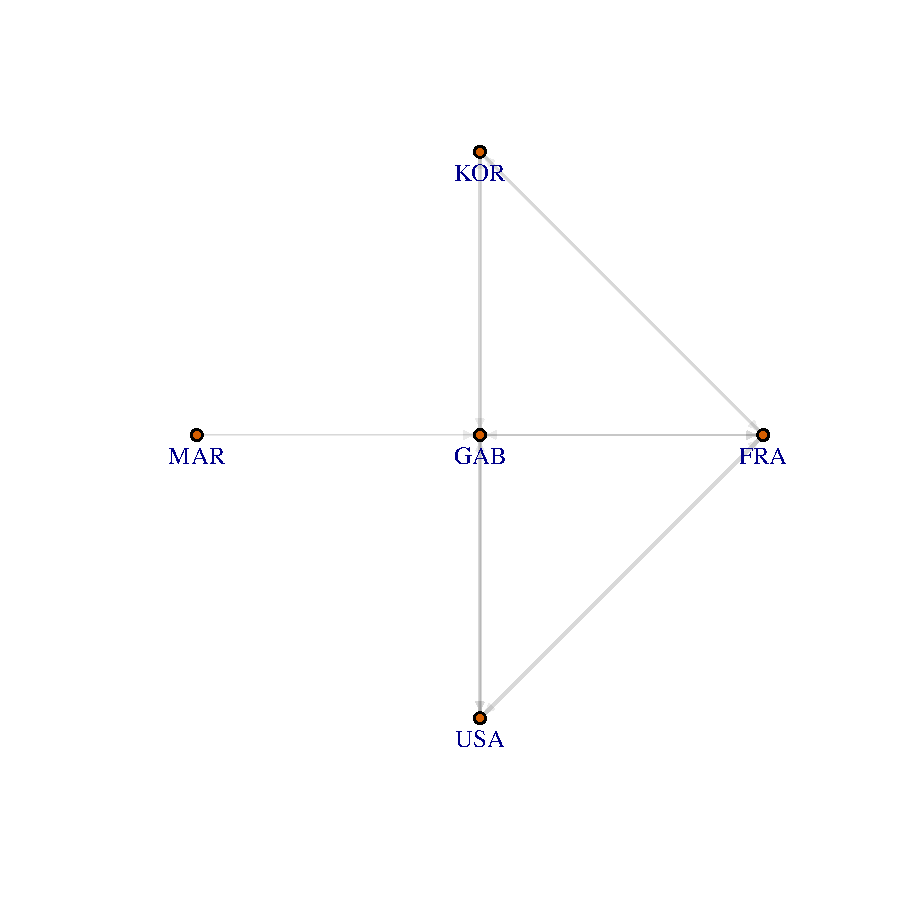
\includegraphics[scale=.7, trim = 1.75cm 1.75cm 1.75cm 1.75cm, clip=true]{figures/GAB2002} &  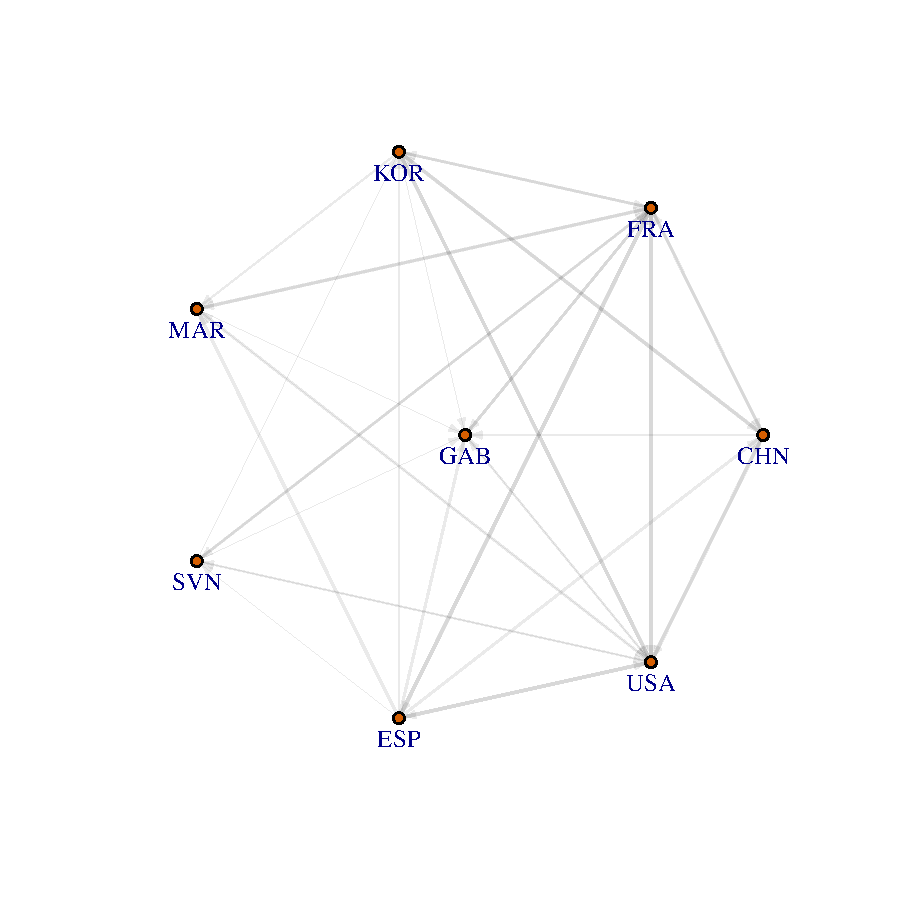
\includegraphics[scale=.7, trim = 1.75cm 1.75cm 1.75cm 1.75cm, clip=true]{figures/GAB2006}  \\\vspace{-.5cm}
%\end{tabular}
%\caption{\label{fig:gab} Networks among Gabon's FDI partners. A state is included in one of these plots if it has either an inward or outward FDI tie with Gabon in the respective year. The width of an edge is proportional to the natural log of the FDI stock value that corresponds to the edge.}
%\end{figure}




\subsection{Covariates}

In the gravity model, we include the log product of the dyad's real GDP\footnote{The data come from the \textit{Penn World Table}  \citep{feenstra2015next}.} and logged Euclidean distance.\footnote{See \citet{mayer2011notes} for the calculation of Euclidean distance.} Generally, higher GDP represents a larger market and therefore should be associated with more FDI, while an increase in geographic distance increases investment costs, decreasing investment flows. For the purpose of model convergence, the logged product of dyadic GDP has been estimated as one variable in the model, rather than being estimated separately. In addition, we include both origin and destination countries' GDP per capita to roughly control for relative factor endowments.\footnote{The data are from the \textit{Penn World Table}.}

Other economic controls include origin and destination countries' trade openness (trade as \% of GDP) and bilateral trade volumes between the origin and destination countries. Existing research has shown that FDI and trade are compliments \citep{aizenman2006fdi,Markusen:1995}. We expect that higher levels of trade openness and bilateral trade will be associated with higher levels of bilateral FDI. Trade openness data are from the World Bank's \textit{World Development Indicators} and trade volume is from the \citet{OECD}.

There is a substantial amount of work that explores the relationship between democratic institutions and FDI inflows; yet empirical results to date remain inconclusive \citep[see,~e.g.,][]{Jensen:2003,Li_Resnick:2003,Jakobsen_DeSoysa:2006,Li_et_al:2018,Wright_Zhu:2018}. We include standard polity scores as a measure of a country's level of democracy \citep{Marshall_Jaggers:2010}. A second institutional variable included is BITs. This binary variable is one if the pair have a stand alone BIT or are party to a preferential trade agreement that also covers investment policy. These treaties should be positively associated with FDI levels as they should effectively remove barriers to investment and provide commitment to liberal economic policies \citep[e.g.,][]{Buthe_Milner:2008,Allee_Peinhardt:2011}. %\citep{Buthe_Milner:2008,buthe2014foreign}.

In addition, we include two sets of international agreement variables. The first is a binary variable for a combination of military alliance treaties that are not defense treaties. The second is a defense treaty. Both are from \citet{Gibler09}. We expect these variables to be positively associated with FDI inflows, particularly defense treaties since this indicates political cooperation and low political risk \citep{Li_Vashchilko:2010}.\footnote{Summary statistics and a correlation matrix of the covariates are provided in Appendix A.}



%The second is preferential trade agreement (PTAs). Signing a PTA represents a commitment to liberal markets that investors would favor and therefore would be associated with increased FDI inflows \citep{Buthe_Milner:2008,buthe2014foreign}. Yet, PTAs vary significantly in depth with some requiring nearly full liberalization of trade barriers while others are superficial political signals. We thus measure the depth of PTAs by using latent trait analysis with 48 different dichotomous variables regarding topics covered in PTAs.\footnote{Data are from \citet{dur2014design}.}






\subsection{Model and Specification: The Count ERGM}

%To model the FDI network, we must use a statistical modeling approach that is capable of representing the dependencies underlying the ties. %The literature offers a number of options. These include the latent space family of models, such as those that have been used to model trade networks in political science \citep{ward2007persistent}; the generalized exponential random graph model (GERGM), which can be used to model complex network features in networks with continuous-valued edges \citep{wilson2017stochastic}; and the ERGM for count-valued edges \citep{krivitsky2012exponential}. We select the count-valued ERGM for two reasons. First, if the researcher's objective is to test hypotheses regarding dependent network structure, ERGM family models can accomplish this more precisely than can latent space models \citep{cranmer2016critique}. Second, the count ERGM offers a modeling advantage over the GERGM for data such as FDI flows, which are zero for the majority of dyads. That is, the count ERGM is capable of modeling zero inflation in the network. This paper presents, as far as we are aware, the first application in political science of the count ERGM proposed by \cite{krivitsky2012exponential}.
Like other forms of the ERGM, the count ERGM is a statistical model that operates on one or more network adjacency matrices. To specify the count ERGM, the researcher selects two types of network statistics---those that relate tie values to observed covariates (i.e., covariate effects), and those that relate the ties to each other via higher-order network structure (i.e., network effects). The ERGM family of models is innovative in that both of these statistic types---covariate effects and network effects, can be included in the same model. Including the network effects helps to accurately identify the true covariate effects \citep{metz2018interdependent}. There are other statistical modeling approaches that could be used to account for network dependence while estimating covariate effects (e.g., latent space methods \citep{matias2014modeling}, stochastic block modeling with covariates \citep{sweet2015incorporating}, and quadratic assignment procedure \citep{robins2012statistical}). However, these alternative methods do not permit precise estimation and testing with respect to specific network effects. Part of our research objective is to test for transitivity and reciprocity effects, so we adopt an ERGM-based approach.

Under \citeapos{krivitsky2012exponential} count ERGM, the probability of the observed $n \times n$ network adjacency matrix $\bm{y}$ is 
\begin{equation}
 \text{Pr}_{\bm{\theta};h;\bm{g}}( \bm{Y}=\bm{y} )=\frac{ h(\bm{y})\text{exp}( \bm {\theta} \cdot \bm{g} (\bm{y}) )}{\bm{\kappa}_{h,\bm{g}}(\bm{\theta})},
 \end{equation}
 where $\bm{g}( \bm{y} )$ is the vector of network statistics used to specify the model, $\bm{\theta}$ is the vector of parameters that describes how those statistic values relate to the probability of observing the network, $h(\bm{y})$ is a reference function defined on the support of $\bm{y}$ and selected to affect the shape of the baseline distribution of dyadic data (e.g., Poisson reference measure), and $\bm{\kappa}_{h,\bm{g}}(\bm{\theta})$ is the normalizing constant.



\subsubsection{Specification}


In the models we specify, we use statistics that model the shape of the individual edge distributions (i.e., the shapes of directed dyadic FDI flows), model the dependencies we have described above, and account for the effects of exogenous covariates. Network statistics in an ERGM model local dependencies, just like conventional covariates, but are expressed at the network-level because that is how they are incorporated into the ERGM probability distribution \citep{desmarais2012micro}. Analogous to selecting covariates to include in a regression model, ERGM software packages present several options for adding network statistics to the model. However, also analogously, the researcher risks overfitting the data if these network statistics are added gratuitously. Specification choices must be guided by theory, and/or strong evidence of specific shortcomings in terms of model fit.  The statistics we use to account for the individual edge distribution include, $$\text{Sum}:\bm{g(y)} = \sum_{(i,j) {\in} \mathbb{Y}}\bm{y}_{i,j},$$ which models the average edge value $$\text{Sum, Fractional Moment}:\bm{g(y)} = \sum_{(i,j) {\in} \mathbb{Y}}\bm{y}_{i,j}^{1/2},$$ which accounts for dispersion in the edge distribution, and
$$\text{Non-Zero}: \bm{g}_k = \sum_{(i,j) {\in} \mathbb{Y}} \mathbb{I}(\bm{y}_{i,j} \neq 0),$$ which models the prevalence of zeros in dyadic FDI flows. We include two statistics to model the dependencies that correspond to our hypotheses. First,
$$ \text{Reciprocity}: \bm{g(y)} = \sum_{(i,j) {\in} \mathbb{Y}}min(\bm{y}_{i,j},\bm{y}_{j,i}),$$ in which we add up the lowest edge value within each dyad. If edges are reciprocated, this statistic will increase due to the co-occurrence of large edge values within the same dyad. Second,
$$\text{Transitive Weights}: \bm{g(y)} =  \sum_{(i,j) {\in} \mathbb{Y}}\min\bigg( \bm{y}_{i,j}, \max\limits_{k{\in}N}\Big(\min(\bm{y}_{i,k},\bm{y}_{k,j})\Big) \bigg),$$ which accounts for the degree to which edge $(i,j)$ co-occurs with pairs of large edge values with which edge $(i,j)$ forms a transitive (i.e., non-cyclical) triad with weighted, directed two-paths going from nodes $i$ to $k$ to $j$. Exogenous covariates are accounted for with statistics that measure the degree to which large covariate values co-occur with large edge values. First,
$$ \text{Dyadic Covariate}: \bm{g(y,x)} = \sum_{(i,j)} \bm{y}_{i,j}x_{i,j},$$ measures this co-occurrence at the level of the directed dyad, in which there is a dyadic observation of the covariate corresponding to each potential FDI flow. There are two statistics that account for node (i.e., country) level covariates. Each statistic takes the product of the node's covariate value and a sum of the edge values in which the node is involved. The first, ``Sender Covariate,'' uses the sum over the edges that the node sends. The second, ``Receiver Covariate,'' uses the sum over the edges that the node receives.

$$ \text{Sender Covariate}: \bm{g(y,x)} = \sum_{i}x_i \sum_{j} \bm{y}_{i,j}$$

$$ \text{Receiver Covariate}: \bm{g(y,x)} = \sum_{j}x_j \sum_{i} \bm{y}_{i,j}$$

The count ERGM estimates that we present below are estimated using the implementation of \citeapos{krivitsky2012exponential} ERGM for count-valued networks made available in the \texttt{ergm.count} \citep{ergmcount} package in the \R \space statistical software. The normalizing constant in the likelihood function for the count ERGM (i.e., the denominator in Equation (1)) is given by $$ \bm{\kappa}_{h,\bm{g}}(\bm{\theta}) =  \sum_{\bm{y} \in \bm{\mathcal{Y} } }  h(\bm{y})\text{exp}( \bm {\theta} \cdot \bm{g} (\bm{y}) ), $$ where $\bm{\mathcal{Y} }$ is the set of all possible count network configurations, and $h(\bm{y}) = \prod_{i,j} (y_{i,j}!)^{-1}$ is the Poisson reference measure, which assures that (1) the normalizing constant is a convergent sum, and (2) produces an edge-wise conditional Poisson distribution if there are no dependence terms in the model. As with the binary ERGM, the normalizing constant in the count ERGM is computationally intractable, and must be approximated. Estimates of $\bm {\theta} $ are calculated using Monte Carlo maximum likelihood (MC-MLE). MC-MLE is an iterative estimation method in which, given starting values for the parameter estimates, Markov Chain Monte Carlo is used to draw a sample of networks to approximate the likelihood function, updated estimates are produced through maximizing the approximate likelihood, and a new sample of networks, drawn using the updated parameters, is generated to approximate the normalizing constant \citep{snijders2002markov}. This iterative process continues until the parameter estimates, and the likelihood function, converge.


We estimate a separate model for each year from 2002 to 2012. We have three main reasons for presenting year-by-year estimates as our main results. First, since analyzing dyadic data essentially squares the size of the data when compared to the monadic level, we have enough data to identify a separate set of parameter values in each year. Second, recent international relations applications have called into question the appropriateness of pooling over long time periods since there may be considerable historical heterogeneity in the parameter values, and have estimated separate models for each year or time period  \citep[see,~e.g.,][]{cranmer2014reciprocity,ward2007persistent}. Third, the appropriateness of a given set of ERGM parameter values is typically specific to the number of nodes in the network \citep{chatterjee2013estimating}, and the number of states in the international system varies slightly over time. In the results we present below, we see that many of the parameters vary considerably over time. In particular, several parameters exhibit significant shifts in magnitude and statistical significance beginning in 2008---a pattern that is likely attributable to the Great Recession. %\footnote{A shift in total FDI flows happens in 2008 as well, as shown in Figure \ref{fig:flows} in the Appendix.}
We present pooled results in Section B in Appendix.


\section{Results}

Throughout the results section, we compare two specifications of the count ERGM---one that assumes conditional independence among the edge values (i.e., the independence model), and the full specification that includes dependence terms. The only two terms that are excluded from the independence model are the reciprocity and transitivity terms. Before discussing individual effects, we first assess the relative fit of the independence and network models. The objective in this fit comparison is to summarize the fit contribution of adding the dependence effects to the model. We are not necessarily searching for the network model that provides the best overall fit to the data---such an exercise would involve the consideration of several other forms of network models. Figure \ref{fig:bic} presents the difference in Bayesian Information Criterion (BIC) in the between the independence and network models for each year in our analysis. We see that the BIC in the independence model is higher than that in the network model for each year, which provides robust evidence that the network model is a better fit for the data than the independence model over the time period that we study.\footnote{One additional consideration with ERGMs regards model degeneracy, based on which nearly all networks drawn from the model will be either completely connected or completely devoid of edges. The models we present are not degenerate, as can be seen from the simulation exercises we present.}


\begin{figure}[!h]
\centering
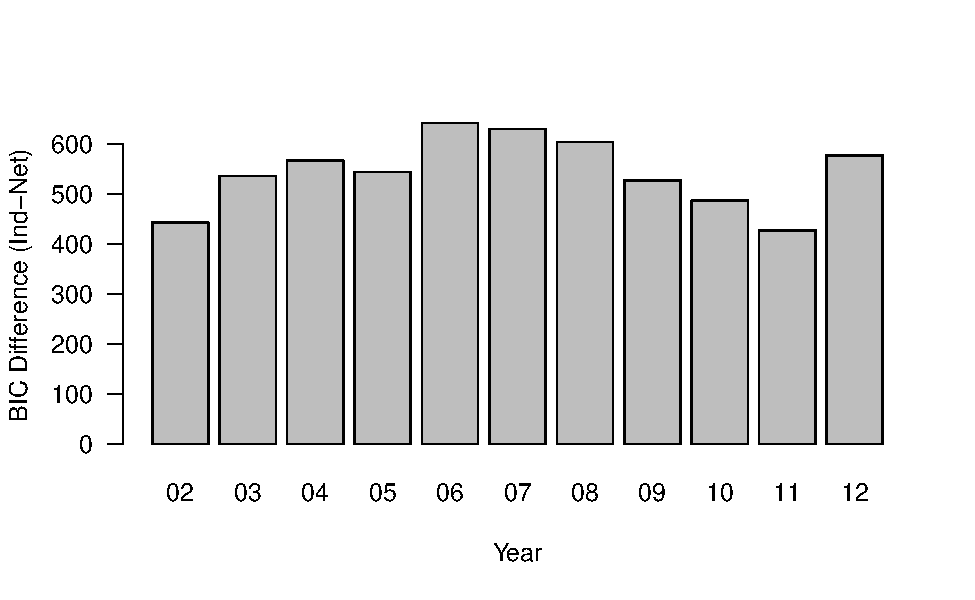
\includegraphics[scale=.75]{figures/BICdiff.pdf} \vspace{-.5cm}
\caption{\label{fig:bic} Difference in BIC between independent and network model.}
\end{figure}


To further illustrate how the network model fits better, and to evaluate different dimensions of the structural fit of the full count ERGM, we compare simulated networks from the two models to the observed networks along four dimensions and for each year.  This is a standard approach to evaluating the goodness of fit of network models \citep[e.g., ][]{krivitsky2008fitting,hunter2008goodness}. We present quantities that evaluate the fit of the models to the reciprocity, transitivity, sender heterogeneity, and receiver heterogeneity of the networks. To measure the fit of the reciprocity, we use the weighted reciprocity measure proposed by \cite{garlaschelli2004patterns}---the correlation between the weights of edges within the same dyads. This measure ranges between -1 and 1, with higher values corresponding to a greater degree of reciprocity.  The measure we use to measure weighted transitivity comes from \cite{opsahl2009clustering}---the ratio of total transitive triple weights to total two-path weights, where the weight of a configuration is defined as the minimum value within the configuration. This measure ranges between 0 and 1, with larger values corresponding to more transitive network. In a perfectly transitive network, large directed tie weights close two-paths that also include two large tie weights.  To measure receiver and sender heterogeneity, we follow \citep{minhas2019inferential} and consider the variance (presented as standard deviations) in the total received (i.e., indegree) and total sent (i.e., outdegree) by each node.

\begin{figure}[!h]
\centering
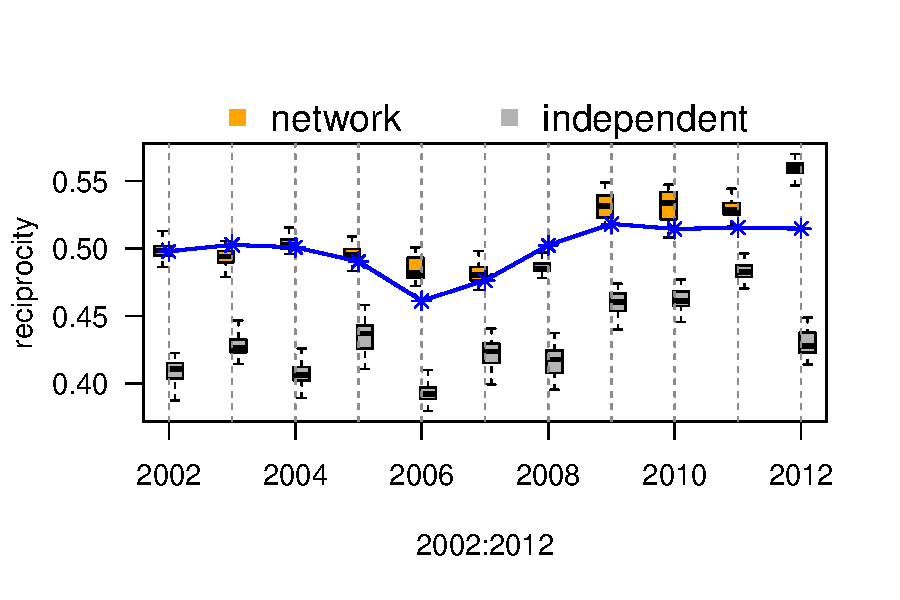
\includegraphics[scale=.75, trim = 0cm 1.5cm .1cm 0cm, clip=true  ]{figures/recip_fit.pdf}  \\
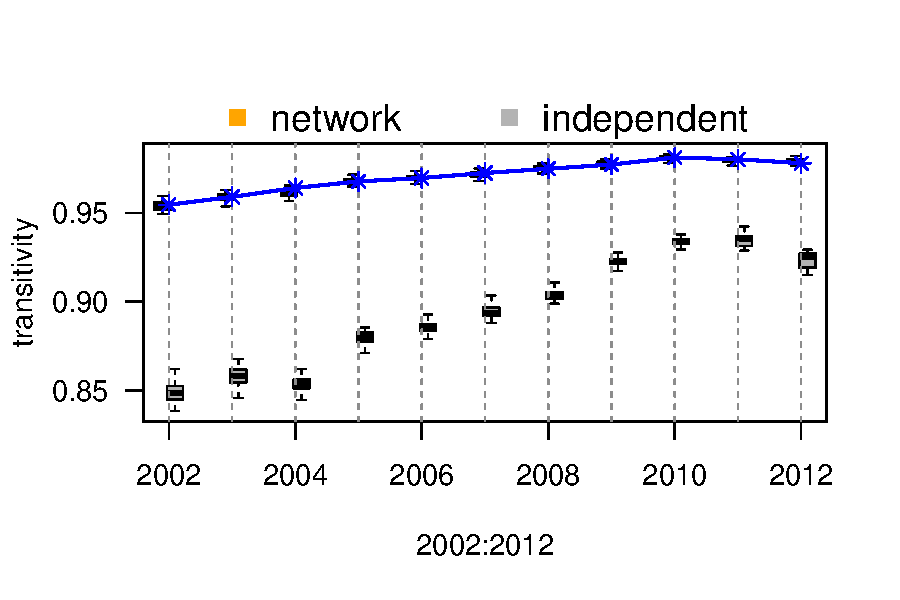
\includegraphics[scale=.75,  trim = 0cm 1.5cm .1cm 2.4cm, clip=true]{figures/trans_fit.pdf}  \\
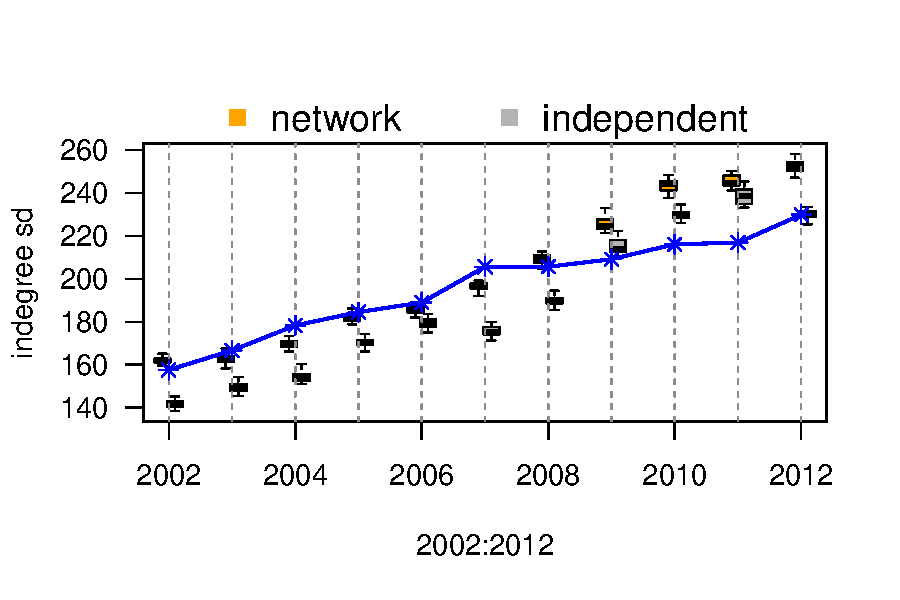
\includegraphics[scale=.75, trim = 0cm 1.5cm .1cm 2.4cm, clip=true]{figures/idsd_fit.pdf}  \\
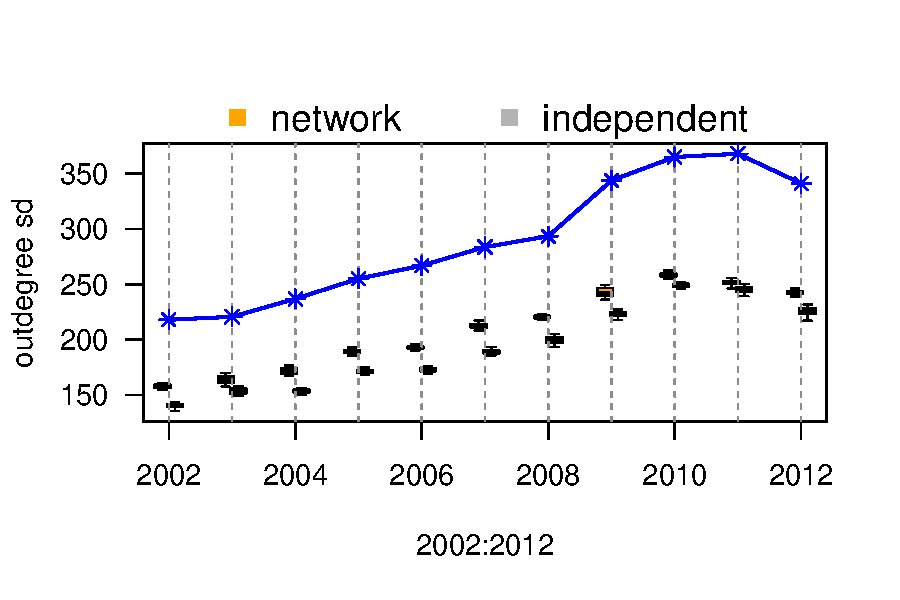
\includegraphics[scale=.75, trim = 0cm 1.5cm .1cm 2.4cm, clip=true]{figures/odsd_fit.pdf} \vspace{-.2cm}
\caption{\label{fig:structureFit} Structural fit of the network and independence models. Boxplots depict distributions over 100 simulated networks. The orange boxplots (those to the left of the dashed vertical lines), depict distributions from the full network model. The gray boxplots (those to the right of the dashed vertical lines) depict distributions from the independence models. The blue-starred lines give the observed values. } 
\end{figure}
We see in Figure \ref{fig:structureFit} that the network model provides a much better fit to the observed network than does the independent model. The boxplots depict the network statistics computed on 100 networks simulated from each model in each year. The network model fits the reciprocity and transitivity in the observed network quite well, and consistently better than does the independence model. The network model generally fits the indegree standard deviation well, but in some years the independent model provides a better fit. The one statistic that is not fit very well with either model is the outdegree standard deviation. Unfotunately, the specifications available for modeling the degree distributions in the count ERGM are still rather limited. The two statistics currently available to model degree heterogeneity---the covariance and square-root-covariance of edge values sent or received by the same node, exhibited degeneracy when fit to the FDI networks. The development of less degeneracy-prone degree statistics, such as the geometrically weighted degree terms available for binary ERGMs \citep{snijders2006new}, is an important avenue for future research with the count ERGM. the observed value is an extreme outlier with respect to the distribution of reciprocity values of networks simulated from the independent model. Unlike the BIC, the fit to the observed structural statistics does not provide a holistic assessment of model fit. Rather, it illustrates the improved fit regarding interpretable quantities calculated on the FDI network, and illustrates how a model in which independence is assumed provides a relatively poor fit in terms of network structure.




Turning now to the network effects, which are presented in Figure \ref{fig:net_effects}, we see that the reciprocity and transitivity effects are positive and statistically significant in each year, offering robust evidence that FDI flows are interdependent according to these two canonical forms of network structure.\footnote{As noted in the Section 3, we also tested our hypotheses on different subsets using different methods of imputation. The majority of these results support our hypotheses, although in the smaller subsets reciprocity is not significant for every year estimated. Since subsetting based on missingness or other variables is not random, this indicates that mutuality is conditional on certain criteria. However, the increase in reciprocity coefficient in later years for most models supports our assertion that reciprocity is becoming more prominent.} While these forms of network dependence are common in networks, they are not inherent and therefore this finding is significant and as substantively important as statistical significance for conventional covariates.
\begin{figure}[htp]
\centering
\begin{tabular}{@{\hskip -.05cm}c@{\hskip -.2cm}c@{\hskip -.2cm}c}
Transitivity  & Reciprocity, OECD pair &Reciprocity, non-OECD pair\\
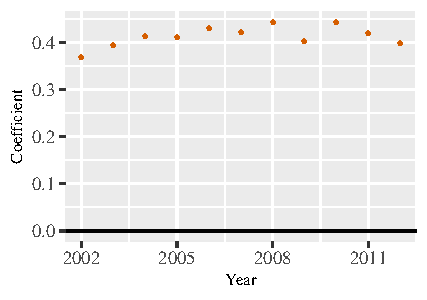
\includegraphics[height=.165\textheight, clip=true, trim=.5cm .5cm 0cm .1cm]{figures/main_rl_plots/Transitivity.pdf}   &
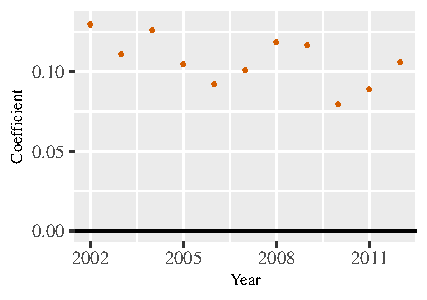
\includegraphics[height=.165\textheight, clip=true, trim=.5cm .5cm 0cm .1cm]{figures/main_rl_plots/Mutuality_OECD.pdf}    &
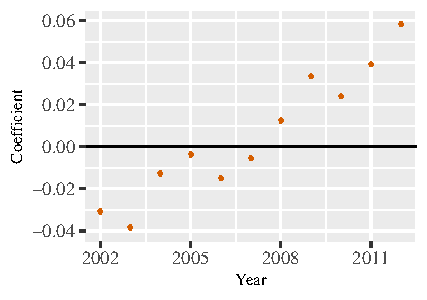
\includegraphics[height=.165\textheight, clip=true, trim=.5cm .5cm 0cm .1cm]{figures/main_rl_plots/Mutuality_notOECD.pdf} \\
\end{tabular}
\caption{\label{fig:net_effects} Estimates of network terms in Poisson ERGMs. Bars span 95\% confidence intervals.}
\end{figure}
The dependence effects, though formulated intuitively, do not permit a straightforward marginal-effects interpretation of the coefficients aside from the signs of the effects. We can, however, estimate and visualize the dependence effects using simulation. In Figure \ref{fig:interpret} we present visualizations of the effects of the dependence terms. To measure these effects we begin with a simulation exercise in which we simulate networks using both the full model with dependence terms, and the null model based only on covariates. We then classify each simulated edge value in terms of the value of the local version of the dependence term operating on that edge. For example, when it comes to the reciprocity effect, we classify each simulated edge value ($y_{i,j}$) in terms of the value of the mutual edge, $y_{j,i}$. Finally, we estimate the difference in means between the edge values simulated from the full and null models at each dependence term value. This difference in means can be interpreted as the effect on predicted edge values of accounting for the respective dependence term in the model.


We see in Figure \ref{fig:interpret}, that the dependence effects can result in differences in predicted edge values in the range of 1--5 in log-scale FDI. The standard deviation in log-scale FDI stock (in 2012---the year we use for the interpretation plots) is 2.40.  We see that the scale of both the reciprocity and transitivity effects are significant, with a shift from lower values of the relevant dependence edge to higher values resulting in more than a standard deviation increase in the predicted edge value.

\begin{figure}[!h]
\centering
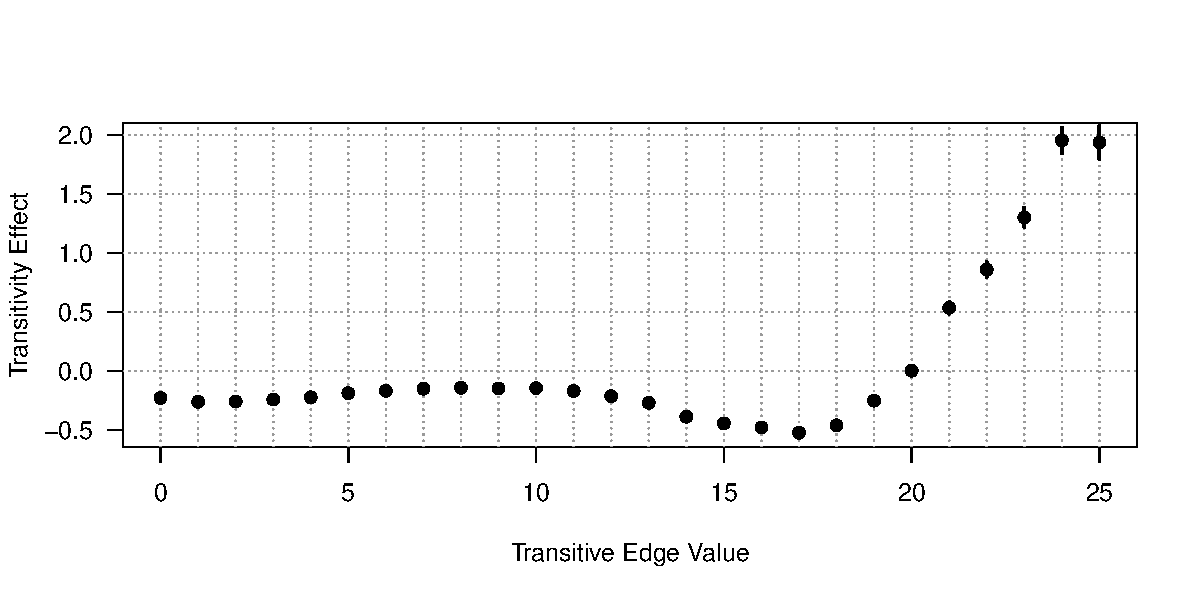
\includegraphics[scale=.75]{figures/transitiveInterpretation.pdf} \vspace{-.5cm}\\
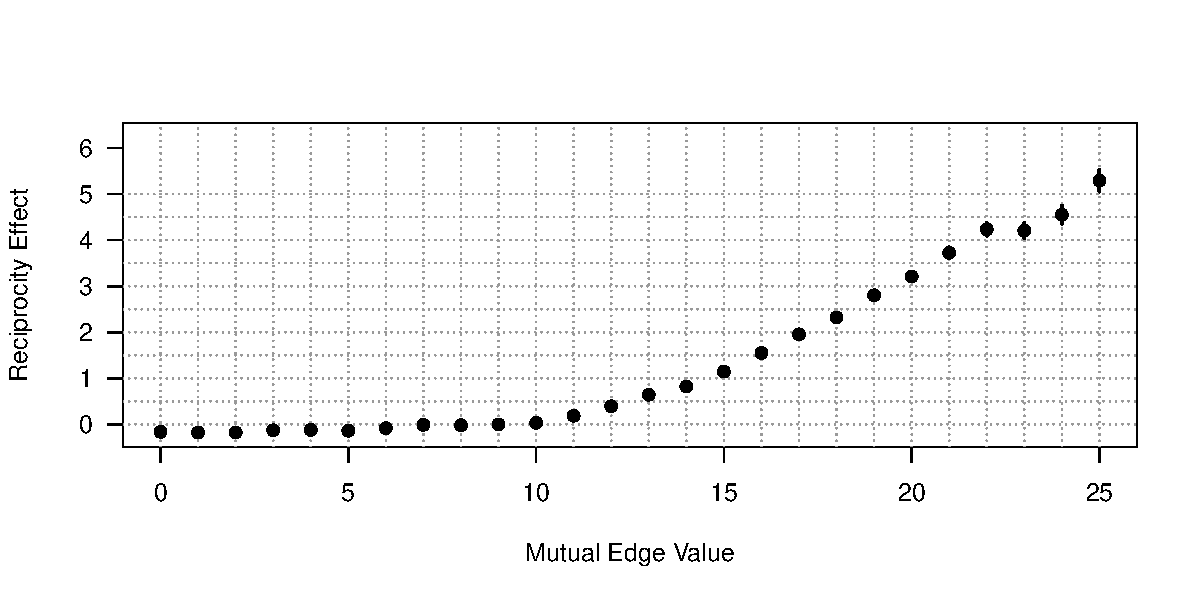
\includegraphics[scale=.75]{figures/mutualInterpretation.pdf} \vspace{-.5cm}
\caption{\label{fig:interpret} Plots depict the difference in predicted value ($y$-axis) that is attributable to the respective dependence effect, averaged over all dyads in the network. Interpretation plots are based on 1,000 FDI stock networks simulated from the 2012 model. Tie weights are measured on the natural logarithm scale. Predicted value differences are calculated by taking the differences between expected dyad values simulated from the full model with dependence terms and the null model that is based on covariates only. Error bars span 95\% confidence intervals for the difference in means. }
\end{figure}




\begin{figure}[htp]
\centering
\begin{tabular}{@{\hskip -.05cm}c@{\hskip -.2cm}c@{\hskip -.2cm}c}
Sum of Edges&
Sum Sqrt. of Edges &
Number of Non-Zero Edges\\
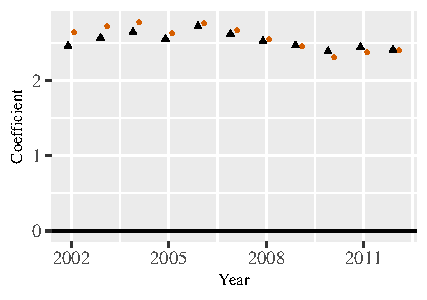
\includegraphics[height=.165\textheight, clip=true, trim=.5cm .5cm 0cm .1cm]{figures/main_rl_plots/Sum.pdf}    &
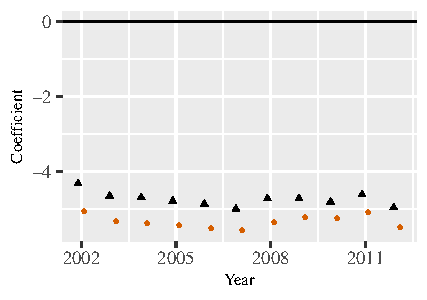
\includegraphics[height=.165\textheight, clip=true, trim=.5cm .5cm 0cm .1cm]{figures/main_rl_plots/Sum_5.pdf}  &
 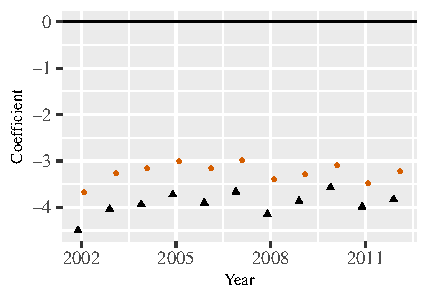
\includegraphics[height=.165\textheight, clip=true, trim=.5cm .5cm 0cm .1cm]{figures/main_rl_plots/Nonzero.pdf}\\
\end{tabular}
\caption{\label{fig:net_controls} Estimates of network control terms in Poisson ERGMs. Bars span 95\% confidence intervals. Black coefficient representations are from models excluding dependence terms (i.e., transitivity and reciprocity). For some models, the confidence intervals are not visible due to being small and the large range of the coefficient estimates.}
\end{figure}

\begin{figure}[htp]
\centering
\begin{tabular}{@{\hskip -.05cm}c@{\hskip -.2cm}c@{\hskip -.2cm}c}

Lagged FDI Flow& 
Log-GDP Product &
Log-Geographic Distance\\

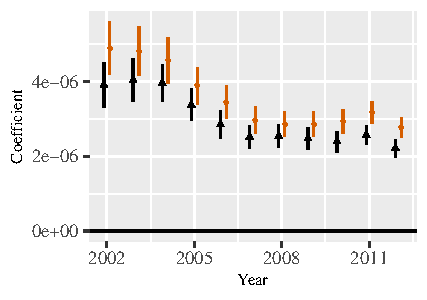
\includegraphics[height=.165\textheight, clip=true, trim=.5cm .5cm 0cm .1cm]{figures/main_rl_plots/LDV.pdf} & 
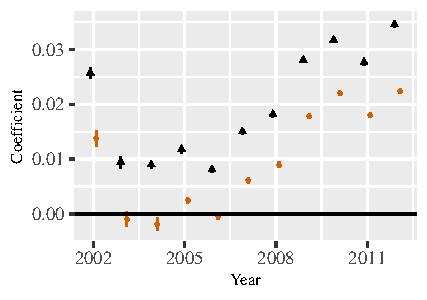
\includegraphics[height=.165\textheight, clip=true, trim=.5cm .5cm 0cm .1cm]{figures/main_rl_plots/Mass.pdf}    &
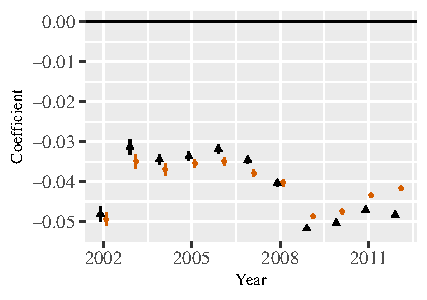
\includegraphics[height=.165\textheight, clip=true, trim=.5cm .5cm 0cm .1cm]{figures/main_rl_plots/Distance.pdf}  \\


Defense Treaty &
Alliance Treaty &
Bilateral Investment Treaty \\

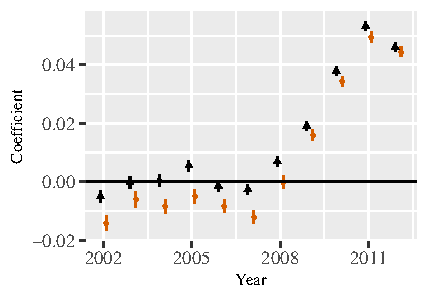
\includegraphics[height=.165\textheight, clip=true, trim=.5cm .5cm 0cm .1cm]{figures/main_rl_plots/Defense_Treaty.pdf}   &
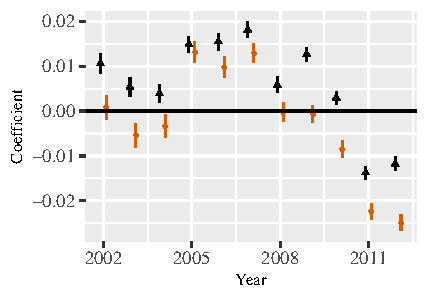
\includegraphics[height=.165\textheight, clip=true, trim=.5cm .5cm 0cm .1cm]{figures/main_rl_plots/Non_Defense_Treaty.pdf} &
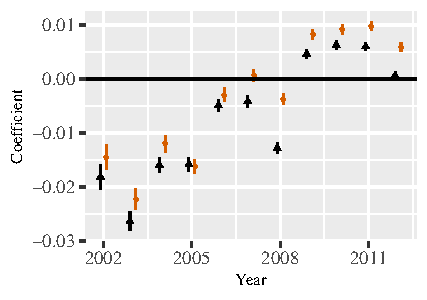
\includegraphics[height=.165\textheight, clip=true, trim=.5cm .5cm 0cm .1cm]{figures/main_rl_plots/Bilateral_Investment_Treaty.pdf}    \\



Bilateral Trade Volume&
OECD membership &
PTA Depth \\


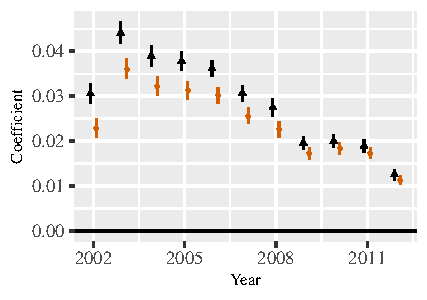
\includegraphics[height=.165\textheight, clip=true, trim=.5cm .5cm 0cm .1cm]{figures/main_rl_plots/Trade_Volume.pdf} &
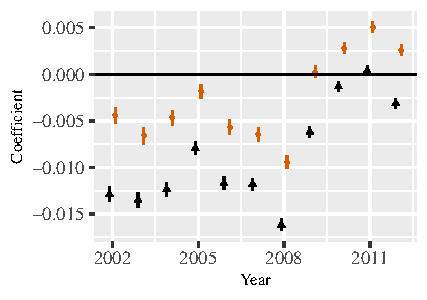
\includegraphics[height=.165\textheight, clip=true, trim=.5cm .5cm 0cm .1cm]{figures/main_rl_plots/Nodematch_OECD.pdf}    &
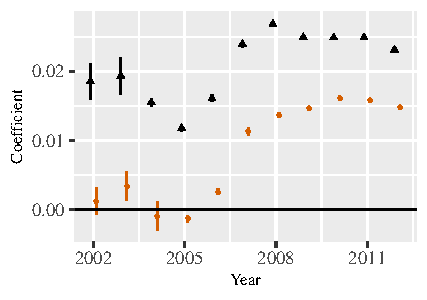
\includegraphics[height=.165\textheight, clip=true, trim=.5cm .5cm 0cm .1cm]{figures/main_rl_plots/PTA_Depth.pdf}    \\

\end{tabular}
\caption{\label{fig:edge_controls} Estimates of exogenous edge terms in Poisson ERGMs. Bars span 95\% confidence intervals. Black coefficient representations are from models excluding dependence terms (i.e., transitivity and reciprocity). For some models, the confidence intervals are not visible due to being small and the large range of the coefficient estimates.}
\end{figure}

\begin{figure}[htp]
\centering
\begin{tabular}{@{\hskip -.05cm}c@{\hskip -.2cm}c@{\hskip -.2cm}c}
Polity, in-degree &
Polity, out-degree &
GDP per capita, in-degree \\
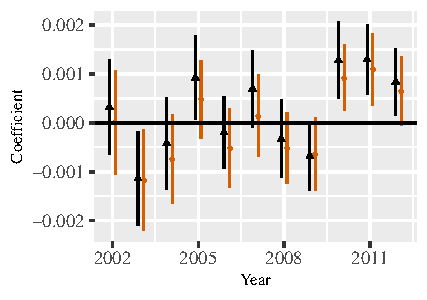
\includegraphics[height=.165\textheight, clip=true, trim=.5cm .5cm 0cm .1cm]{figures/main_rl_plots/Dest_Polity.pdf} &
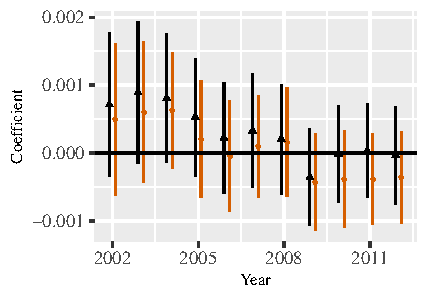
\includegraphics[height=.165\textheight, clip=true, trim=.5cm .5cm 0cm .1cm]{figures/main_rl_plots/Origin_Polity.pdf}  &
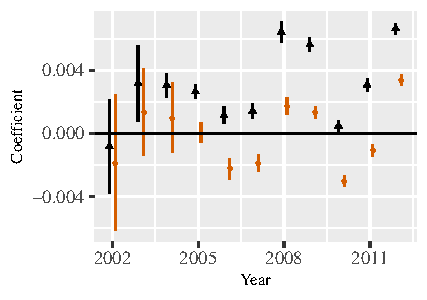
\includegraphics[height=.165\textheight, clip=true, trim=.5cm .5cm 0cm .1cm]{figures/main_rl_plots/Dest_GDPpc.pdf} \\

GDP per capita,  out-degree &
Trade Openness, in-degree&
Trade Openness,  out-degree \\

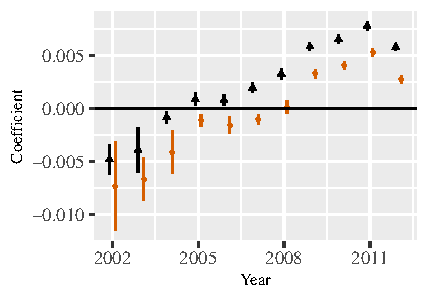
\includegraphics[height=.165\textheight, clip=true, trim=.5cm .5cm 0cm .1cm]{figures/main_rl_plots/Origin_GDPpc.pdf}   &
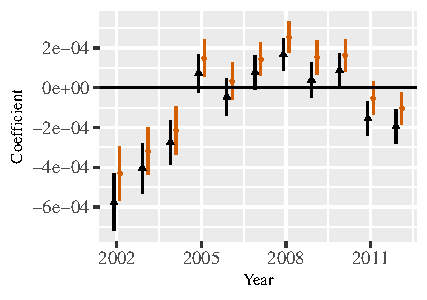
\includegraphics[height=.165\textheight, clip=true, trim=.5cm .5cm 0cm .1cm]{figures/main_rl_plots/Dest_TO.pdf} &
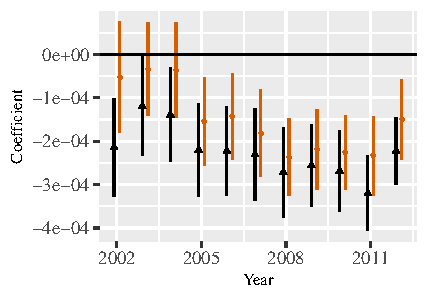
\includegraphics[height=.165\textheight, clip=true, trim=.5cm .5cm 0cm .1cm]{figures/main_rl_plots/Origin_TO.pdf}   \\


\end{tabular}
\caption{\label{fig:node_controls} Estimates of exogenous node terms in Poisson ERGMs. Bars span 95\% confidence intervals. Black coefficient representations are from models excluding dependence terms (i.e., transitivity and reciprocity). For some models, the confidence intervals are not visible due to being small and the large range of the coefficient estimates.}
\end{figure}







Regarding covariate determinants, presented in Table \ref{fig:effectPlots1}, the results show that FDI flows between a dyad are strongly and positively correlated with the product of the dyad's GDP, BIT, defense treaty, both destination and origin countries' polity scores and trade openness, and origin country's GDP per capita. On the other hand, FDI flows are negatively associated with geographic distance between a dyad, alliance treaty, and destination country's GDP per capita. In addition, we see that the coefficient values are not stable over time. Several parameters such as geographic distance, defense treaty, as well as origin and destination's polity scores, GDP per capita, and trade openness change significantly after 2008 when the Great Recession began. The magnitude of most of these coefficients decreases since then. One possible explanation is that concerns about global economic uncertainty might predominate in investment decisions at that time so that home and host countries' political and economic characteristics play a less important role.


We noted above that omitting dependent network structure, a condition that characterizes previous research on FDI, can result in biased estimates and improper standard errors. For several effects that we include in our models, the results are substantively changed by adding the network parameters. In the network model, we find the following effects to be lower in magnitude, statistically significant in fewer years, or both: Gravity model mass, distance, destination polity, destination trade openness, origin trade openness, origin GDP per capita, origin polity, and origin trade openness. For each of these effects, our results indicate that omitting the network dependencies lead to either an overestimate of the effect of the respective variable, or worse, a Type 2 inferential error in which the null hypothesis of no effect is incorrectly rejected. This finding shows that, even if a researcher is not theoretically interested in network dependencies, (s)he should still incorporate them into an empirical model in order to avoid misspecification bias.

\begin{figure}[!h]
\centering
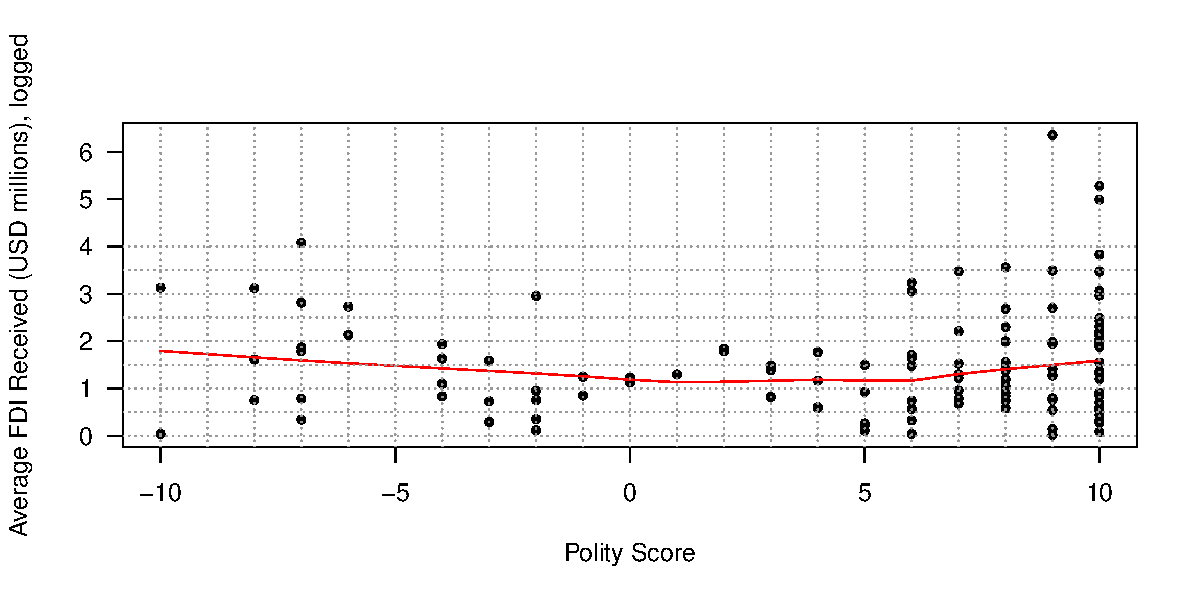
\includegraphics[scale=.75]{./figures/polity_in_sims} \vspace{-.5cm}\\
\caption{\label{fig:polity} Results from the simulation exercise investigating the effects of Polity, in-degree for year 2002. The points are calculated as the the receiver node averages in the adjacency matrix. These results are from 500 simulations. The line in red is the Loess curve.}
\end{figure}

For the Poisson-reference ERGM these covariate estimates are usually interpreted by exponentiating Euler's constant to the power of the coefficient times the number of unit changes in the covariate to get the expected change in the tie weight \citep{krivitsky2013modeling}. Taking Polity, in-degree for example, if the FDI destination had a Polity score of 10 in 2002, we would expect the value of logged FDI being sent to be 1.27 times more than a destination that had a Polity score of -10. In the model with network terms this expected increase is only 1.17 times higher. Another method for interpreting independent terms in the model is to simulate networks using the estimated coefficients while fixing all other independent terms at the mean value and then comparing changes in the average edge value to the range of values of the covariate. For node-level covariates the method is similar. The only change is that you use the column (receiver) averages in the adjacency matrix to compare against covariate values. For illustrative purpose, we present a plot of this for Polity, in-degree below in Figure \ref{fig:polity}. Here the plot shows that as the destination state's Polity increases from the score -10 to the score of 6 there is a slow increase in the average level of FDI received, with a sharper increase between Polity Scores 7 and 10.




\subsection{Ripple Effects of FDI Shocks}\label{contagion}

%When it comes to the analysis of the international political economy,
As we reviewed above, economic contagion has been largely theorized as the ways in which country-level economic conditions can spread through the edges in an economic network. Our analysis reflects a different form of interdependence---characterizing the ways in which the edges in the network depend upon each other. In this section we present an analysis of how a simple shock to the FDI network---the elimination of a single edge---affects the expected values of the edges that are ``close'' to the eliminated edge. The complete elimination of a single FDI edge would be admittedly unlikely, but the effects would be similar to that of a large reduction in an edge value and simulating the network conditional on a fixed but non-zero edge value is much more computationally complex than eliminating an edge entirely. Another way to look at edge elimination is to consider the structural differences we would have observed if a policy was in place to prevent investment along a particular edge (e.g., via an embargo on investment).

We investigate the interdependence in the FDI network by simulating networks from the full model estimated for 2012. Our conclusions are robust to using other years---we use 2012 for consistency with the model interpretations presented above. Our objective in this simulation experiment is to understand how the elimination of an FDI edge from country $i$ to country $j$ affects the other ties to which countries $i$ and $j$ are incident. Specifically, we analyze the effects of eliminating edge $i \rightarrow j$  on four measures: (1) the expected value of FDI ties sent by $i$ to countries other than $j$, (2) the expected value of FDI ties sent by $j$, (3) the expected value of ties received by $i$, and (4) the expected value of ties received by $j$ from countries other than $i$.  These edges are ``close'' to edge $i \rightarrow j$ according to our ERGM specification in that (1) the edge sent from $j$ to $i$ factors directly into the measure of reciprocity, and (2) all edges sent to (from) $i$ and $j$ by other nodes factor into the transitive triads measure with the edge from $i$ to $j$.\footnote{Note that despite including the total amount of investment in the network (via $\text{Sum}:\bm{g(y)}$), the ERGM does not fix the sum of edges in the network---it simply generates networks with, on average, the same value of $\text{Sum}:\bm{g(y)}$ as seen in the observed network. As such, eliminating a single edge from the network will have virtually no effect on the expected values of other edges.}

There are three steps in the simulation experiment we conduct to analyze the effects of eliminating edge $i \rightarrow j$. We first simulate 500 networks from the 2012 ERGM fit. We use this sample to calculate expected values of each edge, as well as our summary measures of indirect effects, from the model without constraints on edge values (i.e., no edges eliminated). Our second step is to, for each observed edge in the 2012 networks, simulate 100 networks from the ERGM with the same parameter values, but with the respective edge value fixed to zero. Our third step is to calculate, again for each edge, the percentage change in the measures of indirect effects that result from eliminating the edge.

\begin{figure}[!h]
\centering
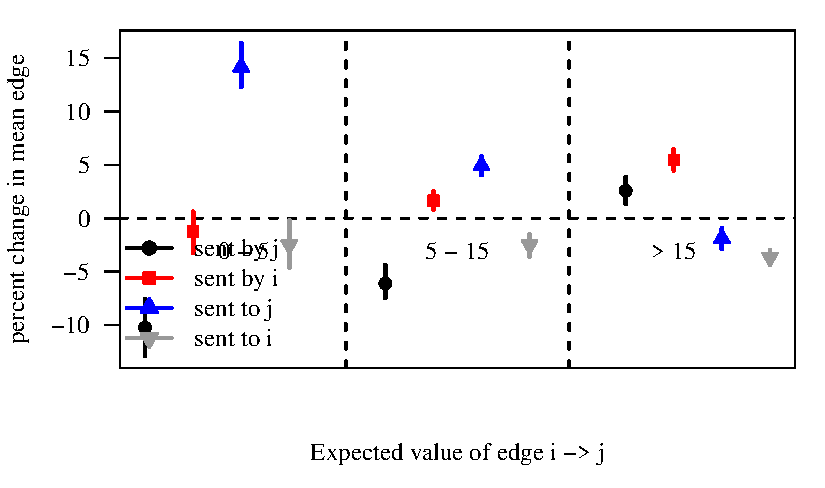
\includegraphics[scale=.85]{./figures/contagion_simulation_results} \vspace{-.5cm}\\
\caption{\label{fig:contagion} Results from simulation exercise investigating the effects of eliminating edge $i \rightarrow j$ on the expected values of other edges incident to both $i$ and $j$. Points are drawn at the average values over all edges in the 2012 network. The bars span 95\% confidence intervals.  Expected values of edges are expressed on the natural logarithm scale.}
\end{figure}

The results from our simulation exercise are presented in Figure \ref{fig:contagion}. We divide the edges in the network into three categories based on their expected values---small edge values (approximately 40\% of edges), between 0 and 5 on the log scale (i.e., \$150m USD or less); medium edge values (approximately 50\% of edges), between 5 and 10 on the log scale (\$150m- \$22bn USD); large edge values (approximately 10\% of edges), greater than 10 on the log scale (\$22bn USD and above). We see that the effects of eliminating small and medium sized edges are mixed. The adverse effects are confined to the sending country $i$ itself. This result could be attributable to the inability to detect domino effects of a relatively small perturbation to the network---the elimination of a single edge---when the edge's value is small. However, as the expected value of the edge being eliminated increases, a consistent signal emerges. For large edges, eliminating edge $i \rightarrow j$ from the network reduces the expected values of other edges sent to/from nodes $i$ and $j$ by 1-2\%. When multiplied over dozens, or even hundreds, of ties to which two countries are incident, a 1-2\% decrease in the value of investments would represent a substantial economic shock. For example, a economic crisis in countries at the center of the network, such as the U.S., will have a ripple effect on FDI inflows and outflows in many other countries with which the U.S. even doesn't have a direct investment tie.









\section{Conclusion}
% paragraph on substantive finding

Since the 1980s, one prominent feature of globalization is that firms have increasingly unbundled and dispersed their activities across the world, leading to the expansion of complex global production networks. One central question is then what accounts for the pattern of cross-border investment flows in the age of complex interdependence. In this paper, we adopt a novel network approach to address this question. %FDI flows represent ties between states that arise through both a complex underlying network of inter and intra-firm relations, and legal agreements between states. The relational backdrop through which FDI operates leads to predictable network structure in the patterns of ties formed through FDI.
We present a network theory of FDI that includes reciprocity and transitivity as the core structural dependencies. We argue that reciprocity arises from the fact that FDI represents an oligopolistic expansion strategy of MNCs and that existing MNCs serve as vehicles for information diffusion and therefore lower the transaction costs for host-country firms to invest in their home countries; Transitivity results from the expansion of global production networks and a safety net created by existing FDI linkages for investors. % and thus facilitates investment flows among countries in the net. 
Empirically, we introduce the ERGM to test our hypotheses. The results of our statistical models confirm that these dependencies exist---a result that holds over time, and while adjusting for other covariates known to relate to FDI.

Our results suggest that in addition to conventional covariates such as factor endowments, market size, and institutional environments, a country's likelihood of receiving FDI depends also on its connections to existing partner states in the network. For example, a country will receive more FDI from the country that its MNCs have have already invested in and from another country when both of them have investment ties with the same third-party country. One policy implication for developing countries is that they should actively attract leading MNCs and integrate themselves into global production networks in order to attract more FDI.

%Our result bears important real-world implications, as network dependencies will lead the effects of policies relevant to FDI to ripple through the network according to these dependencies. In FDI networks, a country's ability to attract foreign investment depends not only on its own locational advantages such as factor endowments, large consumer markets, or favorable government policies, but also on its connectivity to existing partner states in the network. As such, network dependencies will demand more policy coordination among nations, and thus, more likely to promote cooperation and peace \citep[see,~e.g.,][]{Kim_Solingen:2017,Dorussen_Ward:2008,Dorussen_Ward:2010}.


We should emphasize that our theory, specification, and finding of network-wide reciprocity and transitivity represent just the start in a broader scholarly dialogue on the network science of FDI flows. One limitation of our study is that we do not model any forms of conditional variation in reciprocity and transitivity. In theory, we should expect that the degree of reciprocity varies by countries' levels of development. Investing abroad incurs large fixed costs and firms need to overcome the disadvantages such as liability of foreignness they face when competing with indigenous firms in the host country. Therefore, only the most productive firms are able to engage in FDI activities \citep{Helpman_et_al:2004}. Historically, MNCs from developed countries predominate. Although there is a surge of FDI from developing countries since the early 2000s, firms in most developing countries are still not competitive enough to strive in a global market.\footnote{%For instance, in 2005 outward FDI flows and stocks from developing countries are approximately 17\% and 13\% of the world total, respectively \citep{UNCTAD:2006}.
Outward FDI from developing countries is highly concentrated; the top 10 countries, mostly large emerging economies such as Argentina, Brazil, Chile, China, Mexico, Russia, and South Africa contribute about 83\% \citep{UNCTAD:2006}. } It is important to explore how network dependencies vary across different groups of countries.\footnote{In Appendix F, we re-estimate the model by dropping all EU countries to test whether reciprocity and transitivity still hold for the rest of global economy. We find that transitivity remains highly significant and reciprocity becomes either insignificant or negative for earlier years. Our results also show an upward trend in reciprocity over time, which is consistent with the fact that FDI increasingly originates from developing countries. }

Future research could also look into the political and economic consequences of FDI networks. In this article, we take a first step to model the characteristics of FDI networks and show that they exhibit both reciprocity and transitivity. The methodological advancement now allows researchers to examine the effects of the global structure of the network on states. Given the dramatic expansion of global production networks and states are increasingly tied to each other through multinationals' investment activities, it is pivotal to understand the consequences of FDI networks, such as how the networks transmit exogenous shocks, influence domestic politics, and shape international cooperation and conflict.




\newpage
\singlespacing
\bibliographystyle{apsr}
\bibliography{fdi_reference}






\end{document}



Table \ref{tab:describe_binary} provides means for the dichotomous dyadic variables used in our models....

% Table created by stargazer v.5.2 by Marek Hlavac, Harvard University. E-mail: hlavac at fas.harvard.edu
% Date and time: Mon, Feb 20, 2017 - 22:08:59
\begin{table}[htp] \centering
  \caption{}
  \label{}
\begin{tabular}{@{\extracolsep{5pt}}lcccc}
\\[-1.8ex]\hline
\hline \\[-1.8ex]
Statistic &  \multicolumn{1}{c}{Mean} & \multicolumn{1}{c}{St. Dev.} & \multicolumn{1}{c}{Min} & \multicolumn{1}{c}{Max} \\
\hline \\[-1.8ex]
Contiguity &  0.024 & 0.152 & 0 & 1 \\
Common Official Language &  0.112 & 0.315 & 0 & 1 \\
Common Language and Ethnicity &  0.115 & 0.318 & 0 & 1 \\
Former Colonial Relationship &  0.015 & 0.121 & 0 & 1 \\
Common Colonizer &  0.062 & 0.241 & 0 & 1 \\
Defense Treaty &  0.075 & 0.264 & 0 & 1 \\
Non-aggression Treaty &  0.064 & 0.245 & 0 & 1 \\
Neutrality Treaty &  0.004 & 0.063 & 0 & 1 \\
Entente Treaty &  0.066 & 0.248 & 0 & 1 \\
\hline \\[-1.8ex]
\end{tabular}
\caption{\label{tab:describe_binary} Descriptive statistics for dichotomous dyadic covariates. Number of observations across all years is 189,000.}
\end{table}


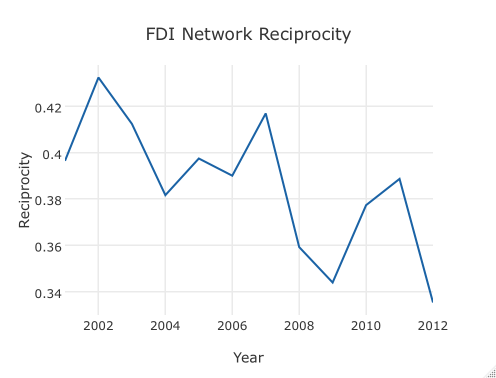
\includegraphics[scale=.8]{figures/reciprocity.png}\\
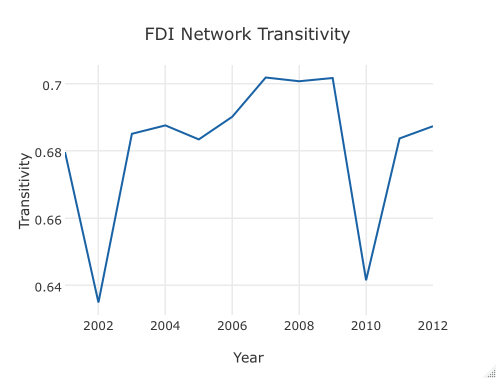
\includegraphics[scale=.8]{figures/transitivity.png}\\
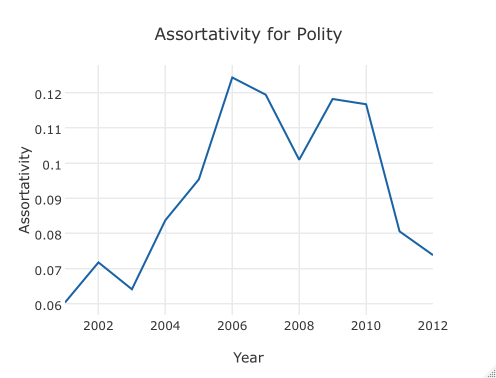
\includegraphics[scale=.8]{figures/assortativity.png}\\
